%% Sets document class
\documentclass[a4paper]{article}

%% Macros
\newcommand{\crmr}{Coordinamento Regionale Malattie Rare}

%% Language and font encodings
\usepackage[italian]{babel}
\usepackage[utf8x]{inputenc}
\usepackage[T1]{fontenc}

%% Sets page size and margins
\usepackage[a4paper,top=3cm,bottom=2cm,left=3cm,right=3cm,marginparwidth=1.75cm]{geometry}

%% Useful packages
\usepackage{graphicx}
\usepackage{float}
\usepackage{hyperref}

%% Long table utilities
\usepackage{longtable}
\usepackage{array}
\newcolumntype{L}[1]{>{\raggedright\let\newline\\\arraybackslash\hspace{0pt}}m{#1}}

%% Subsubsubsection
\usepackage{titlesec}
\titleclass{\subsubsubsection}{straight}[\subsection]
\newcounter{subsubsubsection}[subsubsection]
\renewcommand\thesubsubsubsection{\thesubsubsection.\arabic{subsubsubsection}}
\titleformat{\subsubsubsection}
  {\normalfont\normalsize\bfseries}{\thesubsubsubsection}{1em}{}
\titlespacing*{\subsubsubsection}
{0pt}{3.25ex plus 1ex minus .2ex}{1.5ex plus .2ex}
\makeatletter
\def\toclevel@subsubsubsection{4}
\def\l@subsubsubsection{\@dottedtocline{4}{7em}{4em}}
\setcounter{secnumdepth}{4}
\setcounter{tocdepth}{4}

\begin{document}

\begin{titlepage}

\begin{figure}[H]
	\centering
	
\includegraphics[width=\linewidth]{images/logounipd.jpg}
\end{figure}

\begin{center}
	\LARGE DIPARTIMENTO DI MATEMATICA "Tullio Levi-Civita" \\
    \vspace{5mm}
    \LARGE CORSO DI LAUREA IN INFORMATICA \\
	\vspace{8mm}
    \line(1,0){450} \\
    \vspace{10mm}
    \huge \textbf{Webservices come mezzo di comunicazione tra AUR ed azienda ospedaliera} \\
    \vspace{2mm}
    \LARGE Tesi di laurea triennale \\
\end{center}

\vspace{22mm}

\begin{minipage}[t]{0.50\textwidth}
	{\large{\bf Relatore:}\vspace{1mm} \\ Prof. Ranzato Francesco}
\end{minipage}
\hfill
\begin{minipage}[t]{0.50\textwidth}
	\raggedleft
	{\large{\bf Laureando:} \\ Casagrande Marco \\ }
\end{minipage}

\vspace*{\fill}

\centering{\large{Appello di laurea, 7 dicembre 2017}}

\end{titlepage}

\newpage

\vspace*{\fill}

\begin{center}
	\large{Marco Casagrande: \textit{Webservices come mezzo di comunicazione tra AUR ed azienda ospedaliera}, Tesi di laurea triennale in Informatica, Università degli Studi di Padova, 7 Dicembre 2017}
\end{center}

\newpage

\vspace*{\fill}

\newpage

\listoffigures

\listoftables

\newpage

\tableofcontents

\newpage

\section{Introduzione}
Questo documento vuole esporre il lavoro svolto dallo studente Casagrande Marco durante lo stage presso il \textbf{\crmr}, sotto l'Azienda Ospedaliera di Padova, per la laurea triennale in Informatica. Lo stage è stato svolto e completato con successo nell'arco di trecentosei ore lavorative.
\\ \\
L'azienda ospitante gestisce due applicativi: \textbf{CEDAP} e \textbf{Malattie Rare}. Gli utenti di tali software lavorano nell'ambito sanitario e sono genericamente medici, farmacisti ed infermieri di centri autorizzati. La sezione informatica del \crmr provvede al mantenimento del software, e nel contempo a soddisfare nuove richieste degli utenti. L'azienda svolge anche un ruolo di ricerca nel suo ambito, dunque alcune richieste di modifiche giungono internamente: in generale allo scopo di raccogliere dati statistici. Gli applicativi sono stati acquistati da alcune regioni italiane, tuttavia il mio progetto è confinato alla Regione Veneto in quanto solo questa permette di comunicare con l'\textit{Anagrafe Unica Assistiti Regionale (AUR)\textsuperscript{\hyperref[sec:gl]{G}}}.
\\ \\
L'applicativo CEDAP si occupa del \textit{certificato di assistenza al parto (CEDAP)\textsuperscript{\hyperref[sec:gl]{G}}}. Le attività principali correlate ad esso sono l'inserimento di un nuovo certificato provvisorio/definitivo (in seguito ad una nascita) e la modifica e ricerca di un certificato. Ai fini dello stage, ho interagito esclusivamente con l'attività di inserimento del nuovo \textit{CEDAP\textsuperscript{\hyperref[sec:gl]{G}}}. Le sezioni che ho modificato riguardavano i dati (anagrafici e molti altri) della madre e del padre del/i nuovo/i nato/i.
\\ \\
L'applicativo Malattie Rare si occupa del \textit{certificato di malattia rara\textsuperscript{\hyperref[sec:gl]{G}}} (il cui scopo principale è attestare l'accesso del malato a determinate agevolazioni ed esenzioni) e del registro GH (cui è iscritto chi assume l'ormone della crescita a causa di patologie spesso legate a malattie rare). Le attività principali correlate ad esso sono l'inserimento di un nuovo certificato provvisorio/definitivo (in seguito alla scoperta di una nuova malattia rara nel paziente), la modifica e la ricerca di un certificato, la visualizzazione della malattie rare riconosciute, nonchè la consultazione e la gestione del registro GH. Ai fini dello stage, ho interagito esclusivamente con l'attività di inserimento del nuovo \textit{certificato di malattia rara\textsuperscript{\hyperref[sec:gl]{G}}}, che richiede i dati anagrafici del paziente e molti dettagli riguardanti il suo stato di salute.
\\ \\
La Regione Veneto ha istituito il \textit{progetto SIRV-Interop\textsuperscript{\hyperref[sec:gl]{G}}} per promuovere l'\textbf{e-Government} e l'\textbf{interoperabilità} tra Enti e/o Pubbliche Amministrazioni, da cui è nato il Centro Regionale Servizi di Cooperazione e Interoperabilità (\textit{circuito CReSCI\textsuperscript{\hyperref[sec:gl]{G}}}). All'interno di tale iniziativa, l'\textit{Anagrafe Unica Assistiti Regionale (AUR)\textsuperscript{\hyperref[sec:gl]{G}}} ha schierato una moltitudine di \textbf{webservices} a disposizione di chi ne richiedesse l'accesso. Il \crmr, tramite un elemento informatico chiamato \textbf{porta di dominio}, poteva già accedere ad alcuni servizi esposti dall'\textit{AUR\textsuperscript{\hyperref[sec:gl]{G}}}.
\\ \\
L'obiettivo principale dello stage è stato l'integrazione della funzionalità di chiamata al servizio \textbf{VisureAUR}, in entrambi gli applicativi. La chiamata al servizio sarebbe dovuta avvenire tramite un'\textbf{interfaccia di ricerca}, resa disponibile nelle pagine di inserimento dei dati di madre, padre o paziente, a seconda della situazione. In questo modo, le informazioni anagrafiche, essendo state recuperate direttamente dall'\textit{Anagrafe Unica Assistiti Regionale (AUR)\textsuperscript{\hyperref[sec:gl]{G}}}. sarebbero risultati sperabilmente aggiornati ed esenti da errori. Aggiuntivamente, è stato reputato vitale  il recupero dell'\textbf{IDMPI} del soggetto ricercato, cioè il suo identificatore univoco come paziente, così da sincronizzare il database del \crmr attraverso la \textbf{sottoscrizione} all'\textit{AUR\textsuperscript{\hyperref[sec:gl]{G}}}. Questa procedura permette la ricezione automatica degli aggiornamenti riguardanti le posizioni dei pazienti sottoscritti ed è effettuabile solo comunicando l'IDMPI all'apposito servizio di sottoscrizione dell'\textit{AUR\textsuperscript{\hyperref[sec:gl]{G}}}.

\newpage

\section{Panoramica dell'azienda}
Il \crmr si occupa prevalentemente di quattro mansioni:
\begin{itemize}
	\item la gestione del \textit{certificato di assistenza al parto (CEDAP)\textsuperscript{\hyperref[sec:gl]{G}}};
    \item la gestione del registro GH (ormone della crescita);
    \item la gestione del \textit{certificato di malattia rara\textsuperscript{\hyperref[sec:gl]{G}}};
    \item la ricerca scientifica tramite statistiche riguardanti le tre mansioni sopracitate.
\end{itemize}
Vista l'ampia gamma di tematiche da affrontare, l'azienda al suo interno ospita una buona varietà di specialisti: medici di ogni tipo, farmacisti, psicologi, statistici ed informatici. La sezione informatica, dove ho svolto interamente il mio stage, comprendeva due programmatori ed un sistemista/dirigente.
\\ \\
Lo stage prevedeva l'analisi e la modifica dei due applicativi (CEDAP e Malattie Rare), la modifica del database aziendale e la configurazione della porta di dominio secondo le necessità emerse. I miei interventi sono stati circoscritti a questo dominio ed ho avuto accesso solo alle aree di codice necessarie. Tutto il mio lavoro è stato svolto in un branch della repository SVN aziendale.
\\ \\
Il \crmr dispone di una complessa struttura di reti, dislocata principlamente nelle sedi a Padova (uffici ed ambiente test) e Porto Marghera (ambiente produzione). La procedura standard da seguire per pubblicare un rilascio degli applicativi è il seguente:
\begin{itemize}
	\item ricezione della richiesta (tramite la piattaforma interna Redmine oppure una comunicazione informale);
    \item analisi dei requisiti ed attribuzione della priorità;
    \item progettazione e sviluppo della nuova versione dell'applicativo nell'ambiente di test;
    \item pubblicazione del rilascio dell'applicativo nell'ambiente di clone (cioè una replica dell'ambiente di produzione);
    \item verifica e validazione del nuovo rilascio dell'applicativo (in seguito a correzioni, tornare allo step di progettazione e sviluppo;
    \item pubblicazione finale del nuovo rilascio dell'applicativo nell'ambiente di produzione.
\end{itemize}

\newpage

\section{Presentazione dello stage}

\subsection{Obiettivi dello stage}
Nello stage era inizialmente previsto l'unico obiettivo riguardante l'integrazione degli applicativi con l'\textit{AUR\textsuperscript{\hyperref[sec:gl]{G}}}. Al completamento di esso, viste le molte ore rimanenti, sono stati fissati obiettivi aggiuntivi che continuassero il percorso di esplorazione dei webservices.

\subsubsection{Implementazione di una pagina di ricerca}
In primo luogo avrei dovuto implementare nell'applicativo CEDAP una funzione di ricerca per la madre ed il padre del/i nuovo/i nato/i. Analogamente, avrei dovuto implementare nell'applicativo Malattie Rare una funzione di ricerca per il paziente affetto da malattia rara. L'utente avrebbe potuto accedere alla funzione di ricerca direttamente nella pagina del modulo per il \textit{certificato CEDAP o di malattia rara\textsuperscript{\hyperref[sec:gl]{G}}}.

\subsubsection{Comunicazione con l'AUR tramite la porta di dominio aziendale}
La funzionalità di ricerca avrebbe dovuto usufuire del servizio VisureAUR, esposto espressamente per rispondere a necessità simili dall'\textit{AUR\textsuperscript{\hyperref[sec:gl]{G}}}. Ogni tipo di comunicazione con quest'ultimo deve passare attraverso una porta di dominio, da installare sul webserver del \crmr. La porta di dominio era già installata ma sarebbe stato necessario verificarne l'effettivo funzionamento e configurarla per poterla utilizzare con la mia macchina. Per fruire del servizio VisureAUR, è necessario aver prima stipulato un \textit{accordo di servizio\textsuperscript{\hyperref[sec:gl]{G}}} con il \textit{circuito CReSCI\textsuperscript{\hyperref[sec:gl]{G}}}. Fortunatamente, l'azienda aveva già svolto questa operazione preliminare.

\subsubsection{Archiviazione IDMPI nel database}
Un altro progetto contemporaneo su cui stava lavorando l'azienda, era la sincronizzazione del proprio database con quello dell'\textit{AUR\textsuperscript{\hyperref[sec:gl]{G}}}. A questo scopo, esisteva già un servizio di sottoscrizione, con il quale l'\textit{AUR\textsuperscript{\hyperref[sec:gl]{G}}} invia le posizioni anagrafiche recentemente aggiornate a chiunque sia sottoscritto. Tuttavia, nel database dell'azienda mancava il dato fondamentale del campo IDMPI, cioè l'identificativo (teoricamente) univoco di una persona. Per favorire questo progetto, avrei dovuto recuperare con la ricerca (oltre ai dati anagrafici) l'IDMPI della persona nell'\textit{AUR\textsuperscript{\hyperref[sec:gl]{G}}} ed aggiornarne il record nel database aziendale.

\subsubsection{Autocompletamento del modulo CEDAP/Malattia Rara}
Nel caso l'utente avesse trovato il risultato corretto nella propria ricerca nell'\textit{AUR\textsuperscript{\hyperref[sec:gl]{G}}}, il modulo per il \textit{certificato CEDAP/malattia rara\textsuperscript{\hyperref[sec:gl]{G}}} avrebbe dovuto autocompletarsi coi dati anagrafici ottenuti. Era richiesto che ciò avvenisse nel modo più completo possibile, ad esempio controllando se il luogo di nascita fosse estero, così da escludere a priori l'inserimento manuale in alcuni campi (provincia/regione di nascita).

\subsection{Formazione}
Il tutor aziendale nei primi giorni mi ha presentato la struttura e spiegato brevemente le nozioni più importanti riguardo l'ambito lavorativo. Ad ogni introduzione di un obiettivo aggiuntivo dello stage, il tutor aziendale ha esposto il contesto generale e le richieste che avrei dovuto cercare di soddisfare. Per tutto il tempo, ho potuto consultare qualsiasi membro della sezione informatica in merito a dubbi o problematiche. 
\\
Una volta introdotto all'ambiente di sviluppo, ho potuto osservare tutti i software, le tecnologie e gli strumenti usati dal \crmr, dei quali segue una sintetica esposizione.

\subsubsection{SVN}
SVN è un software open-source di controllo di versione. Il suo scopo è mantenere le versioni correnti e precedenti di qualsiasi tipo di file. SVN offre tutte le classiche operazioni relative a questo genere di software (push, pull, commit, merge) e la possibilità di formare nuovi branch dal trunk.

\subsubsection{Eclipse}
Eclipse è un ambiente di sviluppo software multipiattaforma e multilinguaggio, gratuito ed open-source. Permette di definire degli workspaces e di installare plugins in base alle proprie necessità. 
\\
Al \crmr, Eclipse è presente nella versione Eclipse-Neon ed è integrato con la repository SVN, così da effettuare operazioni di compare e release con modalità semplici e dirette.

\subsubsection{Redmine}
Redmine è un software gratuito ed open-source per la gestione di progetto ed il tracciamento delle richieste. Tramite esso è possibile consultare la wiki del progetto, tenere traccia delle ore lavorative e gestire gli accessi in base al ruolo dell'utente. Permette la visualizzazione del diagramma di Gantt dei vari progetti e può essere integrato con vari software di versionamento.

\subsubsection{WinSCP}
WinSCP è un software gratuito ed open-source sviluppato per il sistema operativo Windows che si occupa principalmente del trasferimento di file da/a computer remoti. Consiste in un client grafico e supporta i protocolli FTP, SFTP ed SCP.

\subsubsection{Apache Tomcat}
Apache Tomcat è un contenitore gratuito ed open-source di Java Servlet. Contiene varie implementazioni delel tecnologie Java Servlet, JavaServer Pages, Java Expression Language e Java WebSocket. Viene usato principalmente come web server per eseguire codice Java.

\subsubsection{Java Server Pages - JSP}
JSP è una tecnologia che permette di eseguire codice Java in pagine web basate su HTML, XML e simili. Presenta una grande simiglianza a PHP ed ASP. Per eseguire le pagine web JSP, è necessaria la presenza di un webserver compatibile (cioè contenente un Servlet Container).

\subsubsection{Java}
Java è annoverato da anni tra i linguaggi di programmazione più diffusi al mondo. E' concorrente, basato sulle classi ed orientato agli oggetti. La sua caratteristica distintiva (almeno originariamente) è quella di essere interpretato a tempo di esecuzione dalla Java Virtual Machine: una macchina virtuale. Grazie a ciò, il codice Java è compatibile con ogni tipo di macchina, indipendentemente dalla sua architettura.

\subsubsection{Javascript}
Il linguaggio Javascript è uno tra i linguaggi di programmazione più utilizzati nello scripting lato client. Javascript è orientato agli oggetti ed agli eventi, tipicamente inserito in pagine HTML, JSP e simili. Essendo debolmente tipizzato e debolmente orientato agli oggetti nonostante sia un linguaggio ad alto livello, permette una grande libertà durante la codifica. Un'altra sua caratteristica di rilievo, è l'essere un linguaggio interpretato e non compilato; l'interprete è direttamente incluso nella maggior parte dei browser (se non in tutti).

\subsubsection{Oracle Database}
Oracle Database è un famoso DataBase Management System (DBMS), cioè un sistema di gestione per database. E' basato sul modello relazionale, che esprime le relazioni tra tabelle in un insieme finito di oggetti, definendone anche vincoli sui valori e le combinazioni di valori possibili.

\subsubsection{XMLdbGUI}
XMLdbGUI è un software gratuito ed open-source che permette la visualizzazione e la consultazione dei database XML tramite interfaccia grafica.

\subsection{Studio preliminare sullo stage}

\subsubsection{Studio di fattibilità}
Una base di partenza per lo studio di fattibilità è stata fornita direttamente dall'azienda. Mi sono stati consegnati due documenti (uno per ogni applicativo) che contenevano considerazioni preliminari riguardo alle potenzialità per il \crmr dall'uso dei webservices esposti dall'\textit{AUR\textsuperscript{\hyperref[sec:gl]{G}}}. In questi documenti era anche contenuta la risposta ufficiale del \textit{circuito CReSCI\textsuperscript{\hyperref[sec:gl]{G}}} che stabiliva i limiti dei parametri che avremmo potuto inviare per la ricerca. Alcuni si sono rivelati particolarmente restrittivi (ad esempio la ricezione di massimo 10 risultati e l'impossibilità di filtrare il sesso o lo status di vita/morte della persona cercata).
//
Inoltre mi è stato fornito un prototipo di richiesta al servizio VisureAUR da configurare per il lavoro autonomo sulla mia macchina. A completare il quadro, il tutor aziendale mi ha introdotto a varie tematiche di rilievo per lo stage ed illustrato le richieste principali che avrei dovuto cercare di soddisfare.
//
L'analisi della documentazione, del contesto aziendale e del codice degli applicativi (in particolare il successo delle mie prove nella richiesta al servizio VisureAUR) mi hanno confermato la possibilità di adempiere alla maggior parte dei requisiti ricavati. I pochi requisiti rimanenti, essendo irrealizzabili per vincoli strutturali ed architetturali, sono stati riadattati o scartati di comune accordo con l'azienda.

\subsubsection{Scadenze}
Lo stage universitario prevede 300-320 ore di lavoro, la cui distribuzione settimanale è definita nel documento del piano di lavoro.
\\
Lo stage ha avuto inizio il 03-07-2017 ed è terminato il 22-09-2017, prevedendo la sospensione del lavoro durante le feste obbligatorie ed un massimo di 3 settimane di vacanze.
\\
Le principali scadenze da rispettare sono state:
\begin{itemize}
	\item la prima stesura dei documenti piano di progetto, norme di progetto, piano di qualifica ed analisi dei requisiti entro il 19-07-2017, così da iniziare puntualmente la fase di progettazione;
    \item la conclusione della fase di codifica entro il 01-09-2017, così da condurre puntualmente i test di sistema, validazione e collaudo, nonchè il rilascio dell'applicativo.
    \item la stesura definitiva di ogni documento sopracitato entro il 22-09-2017, termine ultimo dello stage.
\end{itemize}

\subsection{Pianificazione attività del progetto di stage}

\subsubsection{Definizione attività}
\textbf{Gestione}
\begin{itemize}
	\item Pianificazione e controllo delle attività.
\end{itemize}

\noindent
\textbf{Amministrazione}
\begin{itemize}
	\item Piano di progetto;
    \item Norme di progetto;
    \item Piano di qualifica;
    \item Preparazione dell'ambiente di lavoro.
\end{itemize}

\noindent
\textbf{Analisi}
\begin{itemize}
	\item Studio del dominio;
    \item Esplorazione e formazione sui framework di sviluppo;
    \item Analisi dei requisiti.
\end{itemize}

\noindent
\textbf{Progettazione}
\begin{itemize}
	\item Progettazione architetturale e documentazione;
	\item Progettazione di dettaglio e documentazione.
\end{itemize}

\noindent
\textbf{Sviluppo}
\begin{itemize}
	\item Codifica dei test;
    \item Codifica;
    \item Esecuzione dei test
	\item Stesura del manuale utente.
\end{itemize}

\noindent
\textbf{Verifica e Validazione}
\begin{itemize}
	\item Verifica;
	\item Validazione.
\end{itemize}

\subsubsection{Piano settimanale}
\begin{longtable}{||c|c|L{7cm}|c||}
\hline
Settimana & Periodo indicativo & Programma & Ore \\
\hline
1
& 03/07/17 – 07/07/17
& 
\begin{itemize}
	\item Preparazione dell'ambiente di lavoro;
	\item Pianificazione dettagliata delle attività, prima stesura dei documenti di progetto e del piano di qualifica;
    \item Analisi dei requisiti del sistema, studio dei sistemi informativi già presenti.
\end{itemize}
& 36 \\
\hline
2
& 19/07/17 – 25/07/17
& 
\begin{itemize}
	\item Analisi dei requisiti del sistema e del software;
	\item Definizione dei test di validazione;
    \item Studio dei framework esistenti.
\end{itemize}
& 36 \\
\hline
3
& 26/07/17 – 01/08/17
& 
\begin{itemize}
	\item Progettazione architetturale del sistema;
	\item Definizione dei test di sistema;
    \item Incremento del piano di qualifica, preparazione dell'ambiente di test.
\end{itemize}
& 36 \\
\hline
4
& 02/08/17 – 08/08/17
& 
\begin{itemize}
	\item Progettazione di dettaglio del sistema;
	\item Inizio della codifica dell'applicazione;
    \item Progettazione dei test.
\end{itemize}
& 36 \\
\hline
5
& 09/08/17 – 25/08/17
& 
\begin{itemize}
	\item Codifica dell'applicazione;
    \item Esecuzione dei test;
    \item Incremento dell'analisi dei requisiti a seguito del prototipo.
\end{itemize}
& 36 \\
\hline
6
& 28/08/17 – 01/09/17
& 
\begin{itemize}
	\item Codifica dell'applicazione;
    \item Esecuzione dei test;
    \item Incremento dell'analisi dei requisiti a seguito del prototipo.
\end{itemize}
& 32 \\
\hline
7
& 04/09/17 – 08/09/17
& 
\begin{itemize}
	\item Esecuzione dei test di sistema;
    \item Creazione del manuale d'uso.
\end{itemize}
& 32 \\
\hline
8
& 11/09/17 – 15/09/17
& 
\begin{itemize}
	\item Deployment dell'applicazione;
    \item Esecuzione dei test di validazione.
\end{itemize}
& 32 \\
\hline
9
& 18/09/17 – 22/09/17
& 
\begin{itemize}
	\item Prove di collaudo;
    \item Stesura documenti finali.
\end{itemize}
& 36 \\
\hline
\caption{Tabella del piano settimanale}
\end{longtable}

\subsection{Obiettivi aggiuntivi dello stage}
Il raggiungimento dell'obiettivo di stage è avvenuto più velocemente del previsto, in anticipo di un paio di settimane. Per completare le ore lavorative, assieme al tutor aziendale sono stati stabiliti degli obiettivi aggiuntivi:
\begin{itemize}
	\item configurazione, installazione ed modifiche ad hoc del software ReceiverWS che riceva gli aggiornamenti delle posizioni degli assistiti forniti dalla sottoscrizione all'\textit{AUR\textsuperscript{\hyperref[sec:gl]{G}}};
    \item collegamento di ReceiverWS al database Oracle affinchè, in seguito alla ricezione di nuovi dati, il software li memorizzi automaticamente nel database;
    \item abilitazione del sistema di logging di ReceiverWS affinchè la porta di dominio rilevi e memorizzi le informazioni riguardanti l'esecuzione del software;
    \item progettazione, sviluppo e configurazione di un software SenderWS che esplori le possibilità future per l'invio di dati (in particolare le esenzioni dovute ad una malattia rara), dal \crmr verso l'\textit{AUR\textsuperscript{\hyperref[sec:gl]{G}}};
    \item stesura dettagliata della documentazione riguardante il lavoro effettuato su ReceiverWS, database Oracle e SenderWS.
\end{itemize}

\newpage

\section{Webservices}

\subsection{Definizione di un webservice}
Un webservice è un servizio offerto da una macchina ad un'altra attraverso il web. Tipicamente offre un'interfaccia web che espone un set di operazioni su un database, le quali possono restituire o meno una risposta. La proprietà caratteristica dei webservice è l'interoperabilità: ogni webservice può interagire con un altro, indipendentemente dalla piattaforma di compilazione ed esecuzione e dal linguaggio di programmazione usato.
\\
La comunicazione con un webservice avviene attraverso un protocollo: ad esempio \textit{SOAP\textsuperscript{\hyperref[sec:gl]{G}}}, il classico HTTP od altri. Ogni webservice possiede delle regole per la comunicazione, definite in un file WSDL (Web Services Description Language). Vista la crescente diffusione dei webservices è emersa l'esigenza di architetture standard adatte a supportarli. Con questo scopo, si è molto diffusa la \textit{Service-Oriented Architecture (SOA)\textsuperscript{\hyperref[sec:gl]{G}}}. Parallelamente, l'organizzazione \textit{W3C\textsuperscript{\hyperref[sec:gl]{G}}} lavora da qualche anno alla definizione di uno standard chiamato Webservices Architecture.

\subsection{Procedura standard della chiamata ad un webservice}
\begin{figure}[H]
	\centering
	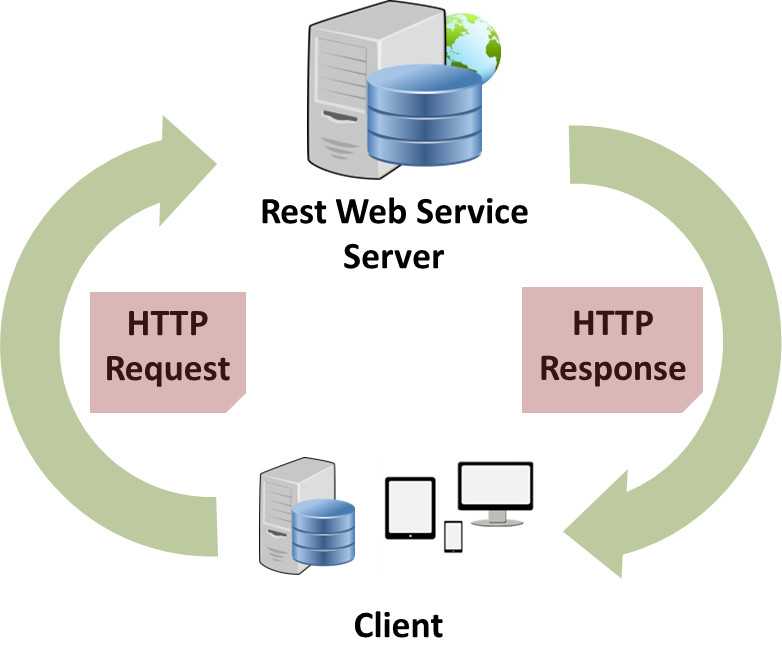
\includegraphics[width=0.4\linewidth]{images/webservice.jpg}
    \caption{Rappresentazione della chiamata ad un webservice RESTful}
\end{figure}
L'interazione con un webservice avviene tra un client ed un server. Il server espone dei servizi al client nel web attraverso un'interfaccia. Il client si collega, con un protocollo adatto, all'endpoint del server, cioè il suo indirizzo di rete, per effettuare una chiamata del webservice. In essa, vengono specificati anche l'operazione da effettuare ed i parametri necessari. Il server esegue internamente l'operazione, inviando una risposta se richiesto dal client. Da notare che il client può essere egli stesso un webservice.

\subsection{Webservices e stage}
Il \textit{circuito CReSCI\textsuperscript{\hyperref[sec:gl]{G}}} definisce come fondamentale il concetto di interoperabilità tra le varie organizzazioni coinvolte. E' naturale che la loro scelta nel creare il progetto di un Servizio Pubblico di Cooperazione Applicativa (SPCoop) sia ricaduta sull'idea di un ampio utilizzo dei webservices all'interno delle porte di dominio. In questo modo è stato possibile separare la responsabilità sui dati interni da quella sui dati immessi nel circuito.
\\
Durante la fase di sviluppo degli applicativi non sono stati impiegati in maniera diretta i webservices, bensì indirettamente nella comunicazione con le porte di dominio (argomento trattato nella prossima sezione). Infatti, per comunicare con la porta di dominio dell'\textit{AUR\textsuperscript{\hyperref[sec:gl]{G}}} è stato utilizzato il servizio VisureAUR.
\\ \\
Riguardo all'obiettivo aggiuntivo del ReceiverWS, la sua implementazione ha preso la forma di una libreria installata nella porta di dominio. Quest'ultima resta in ascolto di eventuali messaggi al servizio MDB-PLS-WS e comunica con la porta di dominio dell'\textit{AUR\textsuperscript{\hyperref[sec:gl]{G}}} tramite webservices. Tuttavia il software di base fornitoci dai responsabili informatici del \textit{circuito CReSCI\textsuperscript{\hyperref[sec:gl]{G}}} comprende un wrapper che si occupa autonomamente della ricezione dati. Anche in questo campo, il rapporto con i webservices è stato indiretto. 
\\ \\
Riguardo all'obiettivo aggiuntivo del SenderWS, la sua implementazione ha preso la forma di un webservice e del corrispondente client. Per la comunicazione con la porta di dominio, ho potuto riusare parte del codice già presente nella funzione di ricerca sviluppata negli applicativi. Il webservice è stato sviluppato tramite Eclipse, che ha generato automaticamente il client.
\\ \\
Lo studio dei webservices e la precedente esperienza durante il progetto di Ingegneria del Software si sono rivelate molto utili per comprendere i meccanismi interni della porta di dominio. Una modesta parte dello stage consisteva nella valutazione personale su come implementare determinati comportamenti, effettuando scelte ragionate e motivandole.

\newpage

\section{Porta di dominio}

\subsection{Definizione di porta di dominio}
La porta di dominio è un ente informatico che delimita il confine del dominio, cioè lo spazio di responsabilità dell'ente erogatore/fruitore di un servizio e lo spazio di trasporto. Le informazioni all'interno della porta di dominio sono di responsabilità dell'ente proprietario, mentre quelle che circolano all'esterno sono prese in carico dal circuito di trasporto. La porta di dominio fa parte del progetto \textit{SIRV-Interop\textsuperscript{\hyperref[sec:gl]{G}}} nella quale è collocato il \textit{circuito CReSCI\textsuperscript{\hyperref[sec:gl]{G}}}.
\\
La porta di dominio è suddivisa in due componenti:
\begin{itemize}
	\item la \textbf{porta applicativa} che espone i propri servizi (alle porte delegate) e quindi svolge il ruolo di fornitore dei servizi;
    \item la \textbf{porta delegata} che invia richieste a servizi esterni (esposti dalle porte applicative) e quindi svolge il ruolo di fruitore dei servizi.
\end{itemize}

\subsection{Porta di dominio e stage}
Le porte di dominio sono un elemento fondamentale per l'interoperabilità e la comunicazione all'interno del \textit{circuito CReSCI\textsuperscript{\hyperref[sec:gl]{G}}}. Sia il \crmr che l'\textit{AUR\textsuperscript{\hyperref[sec:gl]{G}}}, operando in ambito sanitario, aderiscono al Servizio pubblico di cooperazione applicativa (SPCoop) e possiedono una propria porta di dominio.
\\
Durante lo stage sono intervenuto più volte all'interno della configurazione della porta di dominio installata dal \crmr. Prima durante lo sviluppo di ReceiverWS, il quale necessitava di essere installato come libreria nella porta di dominio dell'azienda. Poi al momento della creazione del servizio MDB-PLS-WS per la ricezione degli aggiornamenti sulle posizioni degli assistiti.
\\
La struttura della porta di dominio si è rivelata molto complessa, in quanto deve accontentare un svariate necessità ed ha bisogno di una buona dose di configurazione manuale. Sfortunatamente, il supporto della documentazione e del responsabile del \textit{circuito CReSCI\textsuperscript{\hyperref[sec:gl]{G}}} ha lasciato a desiderare. La documentazione non era aggiornata ed il responsabile ha commesso alcune leggerezze, nonostante la sua tempestività ed ampia conoscenza del campo. Altri problemi considerevoli sono spuntati dalla necessità di analizzare la struttura della rete aziendale al fine di configurare i nuovi servizi della porta di dominio.

\newpage

\section{SPCoop}

\subsection{Definizione SPCoop}
SPCoop è un modello contenente le modalità tecniche per l’interoperabilità e la cooperazione applicativa, la qualificazione delle componenti infrastrutturali SPCoop e l’utilizzo dei Servizi di Infrastruttura per l’Interoperabilità, la Cooperazione Applicativa e l’Accesso (SICA).

\subsection{SPCoop e stage}
Un tema spinoso con cui mi sono confrontato già durante lo studio di fattibilità è stato il meccanismo di comunicazione tra le porte di dominio. Per comprenderlo, occorreva imparare cosa fosse il modello SPCoop.
\begin{figure}[H]
	\centering
	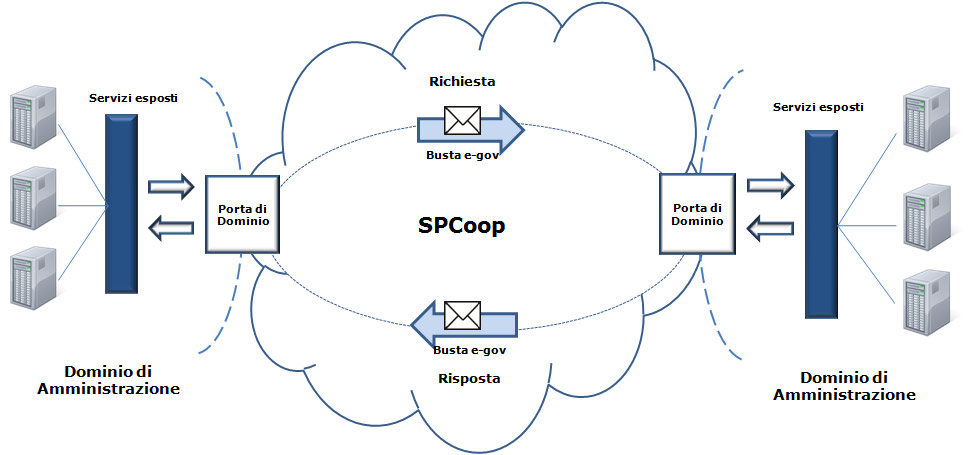
\includegraphics[width=0.4\linewidth]{images/SPCoop.jpg}
    \caption{Servizio Pubblico di Cooperazione Applicativa - SPCoop}
\end{figure}
Le porte di dominio si affacciano alla rete SPCoop, ognuna esponendo i propri servizi come definito negli \textit{accordi di servizio\textsuperscript{\hyperref[sec:gl]{G}}} con altre porte di dominio. Senza un \textit{accordo di servizio\textsuperscript{\hyperref[sec:gl]{G}}} non è possibile usufruire dei servizi esposti. Quando due reti vogliono comunicare, spediscono le informazioni tramite la propria porta delegata. Il messaggio viene avvolto in una \textit{busta e-Gov\textsuperscript{\hyperref[sec:gl]{G}}} e transita nella rete SPCoop giungendo alla porta applicativa del destinatario. La porta di dominio del destinatario rispedisce al mittente l'acknowledgement con eventuali errori o risposte. Il messaggio contenuto nella \textit{busta e-Gov\textsuperscript{\hyperref[sec:gl]{G}}} deve rispettare lo standard internazionale sanitario \textit{HL7\textsuperscript{\hyperref[sec:gl]{G}}}.
\\
Nell'ambito delle attività di stage, sono stati affrontati entrambi gli scenari di fruizione tramite porta delegata ed erogazione tramite porta applicativa.

\newpage

\section{Applicativi CEDAP / Malattie Rare}

\subsection{Richieste dell'azienda}
Il lavoro sugli applicativi mantenuti dal \crmr è stato il cuore del progetto. L'adempimento degli obiettivi su di essi, adattandoli in corso d'opera in caso di imprevisti, costituiva il minimo necessario per un esito positivo dello stage.
\\
Nonostante gli applicativi CEDAP e Malattie Rare presentassero profonde differenze in scopo, utilizzo e struttura, durante l'esposizione del progetto di stage verranno considerati come un unico agglomerato. I settori del codice software interessati dal mio intervento erano comuni ai due applicativi e le differenze tra essi sono stati minime. In ogni caso, non avrebbe avuto senso implementare la stessa funzionalità nei due applicativi secondo modalità differenti. Le differenze realmente rilevanti, sono comunque state indicate nella trattazione seguente.
\\
La necessità di instaurare un canale di comunicazione tra l'azienda e l'\textit{AUR\textsuperscript{\hyperref[sec:gl]{G}}} deriva dalla volontà di:
\begin{itemize}
	\item semplificare l’inserimento dei dati da parte delle varie tipologie di utenti;
    \item migliorare la qualità dei dati del \crmr, fonte di importanti dati statistici;
    \item abilitare l’ottimizzazione e l’automazione di diversi processi interni agli applicativi ed all'azienda.
\end{itemize}
Per conseguire tali benefici, il \crmr ha ritenuto che l'integrazione degli applicativi con i webservices offerti dall'\textit{AUR\textsuperscript{\hyperref[sec:gl]{G}}} fosse la via corretta da seguire.
\\
Durante il progetto sono stati dunque affrontati i seguenti punti salienti:
\begin{itemize}
	\item studio ed analisi critica dei webservices offerti dall'\textit{AUR\textsuperscript{\hyperref[sec:gl]{G}}};
    \item configurazione dell'applicativo per la comunicazione con l'\textit{AUR\textsuperscript{\hyperref[sec:gl]{G}}};
    \item valutazione di possibili miglioramenti rispetto alle richieste minime dell'azienda (particolare interesse per l'uso del campo IDMPI).
\end{itemize}

\subsection{Definizione degli obiettivi}
Le richieste dell'azienda sono state molto flessibili riguardo alle modalità di implementazione delle nuove funzionalità. Come punto di partenza il tutor aziendale mi ha fornito il codice di un tentativo passato di comunicazione con l'\textit{AUR\textsuperscript{\hyperref[sec:gl]{G}}}. Studiando quest'ultimo e gli applicativi, ho cominciato ad estrapolare i requisti dalle richieste.
\\
Per semplificare l'accesso e l'inserimento dei dati da parte degli utenti, ho scelto l'implementazione di una funzione di ricerca durante la compilazione del \textit{CEDAP\textsuperscript{\hyperref[sec:gl]{G}}} o del \textit{certificato di malattia rara\textsuperscript{\hyperref[sec:gl]{G}}} (in base all'applicativo considerato). In questo modo, con l'immissione di pochi specifici dati anagrafici del paziente, è possibile ricavarne molti altri direttamente dall'\textit{AUR\textsuperscript{\hyperref[sec:gl]{G}}}. Ciò permette all'utente di evitare la lunga e tediosa compilazione manuale, raggiungendo il livello di automazione desiderato dall'azienda.
\\
Il miglioramento della qualità dei dati a disposizione del \crmr risulta immediato nel caso si compili sempre il modulo del certificato con i dati recuperati dall'\textit{AUR\textsuperscript{\hyperref[sec:gl]{G}}}. Nonostante questi a volte possano dimostrarsi poco aggiornati, sono comunque la fonte ufficiale più affidabile a disposizione e dovrebbero essere il principale punto di riferimento per l'ambito sanitario. 
\\
Esiste la possibilità di una futura sottoscrizione all'\textit{AUR\textsuperscript{\hyperref[sec:gl]{G}}} così da mantenere una costante conformità dei dati nel database aziendale. In vista di tale sviluppi, ho provveduto a ricavare il campo IDMPI del soggetto ricercato. Ad ogni ricerca, se il soggetto non è presente nel database aziendale, oppure è presente ma è sprovvisto di campo IDMPI, tale dato verrà inserito assieme ad eventuali ulteriori aggiornamenti.
\\
Ho posto dei vincoli su alcune informazioni fondamentali del paziente (nome, cognome, codice fiscale, data di nascita, luogo di nascita) che non potranno mai essere modificate. In caso contrario, si sarebbe creata una situazione con dati anagrafici misti mentre l'idea è di separarli in base al tipo di completamento (inserimento manuale o per ricerca). Le informazioni più volatili, come il numero di telefono della residenza, possono invece essere modificate dall'utente anche se ottenute dall'\textit{AUR\textsuperscript{\hyperref[sec:gl]{G}}}.
\\
Nell'ottica di estensioni future, ho posto particolare attenzione alla lettura delle informazioni ottenute dal servizio VisureAUR. Il messaggio di risposta è espresso nello standard sanitario \textit{HL7\textsuperscript{\hyperref[sec:gl]{G}}} ed è contenuto in una busta \textit{e-Gov\textsuperscript{\hyperref[sec:gl]{G}}}. Attualmente la maggior parte dei campi della risposta sono superflui agli scopi degli applicativi ma ciò potrebbe variare nel tempo. Ogni tag \textit{HL7\textsuperscript{\hyperref[sec:gl]{G}}} presenta sostanziali differenze ed è stato necessario analizzare la procedura di lettura adeguata a ciascun dato importante. Essendo questa la parte più disorientante del codice scritto, ho inserito commenti particolarmente dettagliati ad ogni passaggio.
\\
In conclusione, gli obiettivi dello stage riguardo agli applicativi CEDAP e Malattie Rare sono stati:
\begin{itemize}
	\item l'implementazione di una pagina di ricerca (per madre, padre e paziente);
    \item la configurazione della comunicazione con l'\textit{AUR\textsuperscript{\hyperref[sec:gl]{G}}} tramite la porta di dominio dell'azienda;
    \item la ricezione e l'archiviazione dell'IDMPI di madre, padre o paziente nel database dell'azienda;
    \item l'autocompletamento del modulo CEDAP e Malattia Rara in base alle informazioni ricevute dall'\textit{AUR\textsuperscript{\hyperref[sec:gl]{G}}}.
\end{itemize}

\subsection{Lavoro svolto sugli applicativi}

\subsubsection{Panoramica del control flow}
Vista l'ampia estensione degli applicativi, presento solo una panoramica delle situazioni più rilevanti e frequenti alle quali ho lavorato.
\\
Per una descrizione dettagliata dei casi d'uso e dei requisiti individuati durante il lavoro sugli applicativi, consultare la sezione \textit{Appendice\textsuperscript{\hyperref[sec:ap]{A}}} in fondo a questo documento.

\subsubsubsection{Compilazione della sezione Madre APP-CEDAP}
\begin{figure}[H]
	\centering
	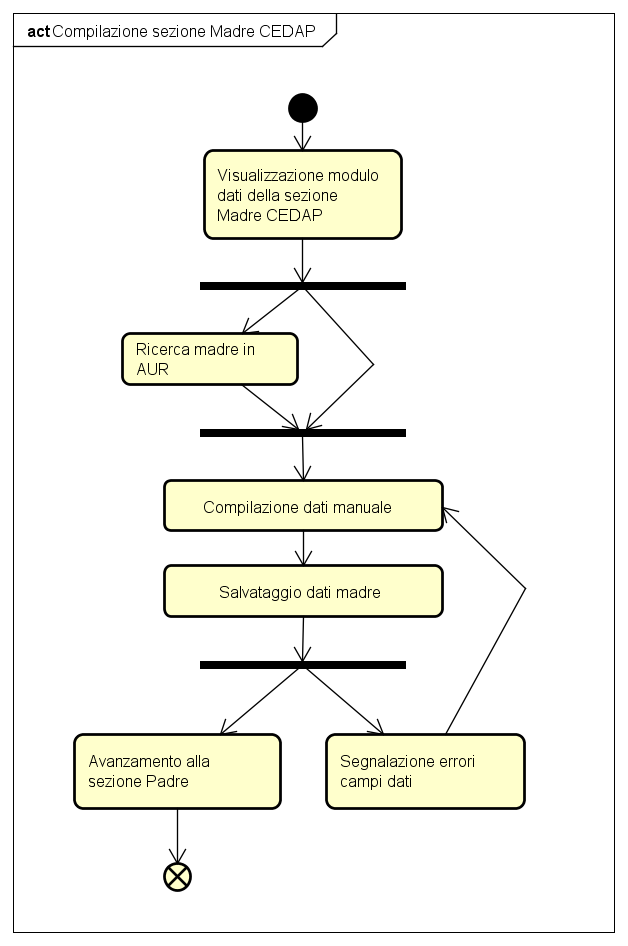
\includegraphics[width=0.4\linewidth]{uml/sezionemadrecedap.png}
    \caption{Diagramma di attività - Compilazione sezione madre CEDAP}
\end{figure}
Dalla schermata principale dell'applicativo CEDAP, è possibile passare alla schermata di compilazione di un nuovo CEDAP. In tale pagina sono presenti una moltitudine di campi dati da compilare, sia obbligatori che facoltativi. Tutte queste informazioni riguardano la madre del nuovo nato, sono perlopiù di tipo anagrafico e vengono attualmente inserite dall'utente. Come alternativa a ciò, ho introdotto la funzione di ricerca della madre nell'\textit{AUR\textsuperscript{\hyperref[sec:gl]{G}}}, attraverso la quale i campi dati vengono compilati automaticamente con le informazioni a disposizione della Regione Veneto. Terminata la compilazione, è possibile salvare i dati (comunque modificabili successivamente) e procedere alla sezione padre del CEDAP.
\\
La sezione padre del CEDAP è molto simile a quella della madre, anche se necessita di meno informazioni. Diversamente, la procedura per il \textit{certificato di Malattia Rara\textsuperscript{\hyperref[sec:gl]{G}}} di un paziente richiede un insieme diverso di informazioni e consiste in una singola sezione. Nonostante questa osservazione, viene applicata la stessa logica di fondo dunque non sono necessari ulteriori approfondimenti.

\subsubsubsection{Ricerca della madre APP-CEDAP}
\begin{figure}[H]
	\centering
	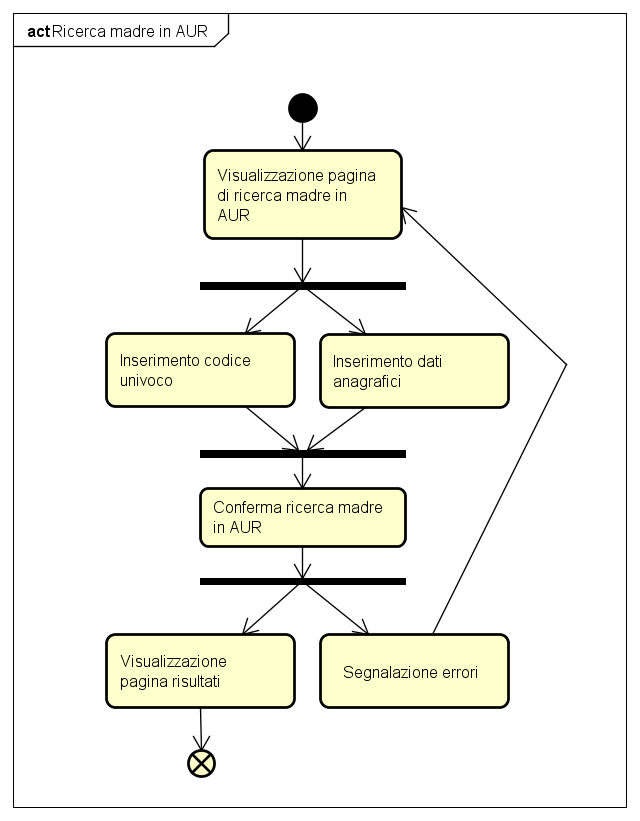
\includegraphics[width=0.4\linewidth]{uml/ricercamadreaur.png}
    \caption{Diagramma di attività - Ricerca madre CEDAP}
\end{figure}
Dalla schermata di compilazione del nuovo CEDAP, è possibile passare alla schermata di ricerca della madre del nuovo nato. Le possibilità di ricerca sono due:
\begin{itemize}
	\item per codice identificativo univoco (codice fiscale, STP ENI o TEAM);
    \item per dati anagrafici (nome e cognome obbligatori, data di nascita consigliata, luogo di nascita opzionale).
\end{itemize}
Confermata la ricerca, la richiesta viene inoltrata all'\textit{AUR\textsuperscript{\hyperref[sec:gl]{G}}} ed un indicatore visivo segnala lo stato di attesa. Ricevuta la risposta con i risultati, si viene reindirizzati alla pagine con la lista ordinata. Da lì è possibile scegliere uno dei risultati come madre, tornando al modulo CEDAP ed autocompletandolo, oppure eseguire una nuova ricerca.
\\
La ricerca del padre di un nuovo nato e di un paziente affetto da malattia rara fruiscono allo stesso modo del servizio VisureAUR, dunque non possiedono differenze significative dalla ricerca della madre di un nuovo nato.

\subsubsubsection{Chiamata alla porta di dominio}
\begin{figure}[H]
	\centering
	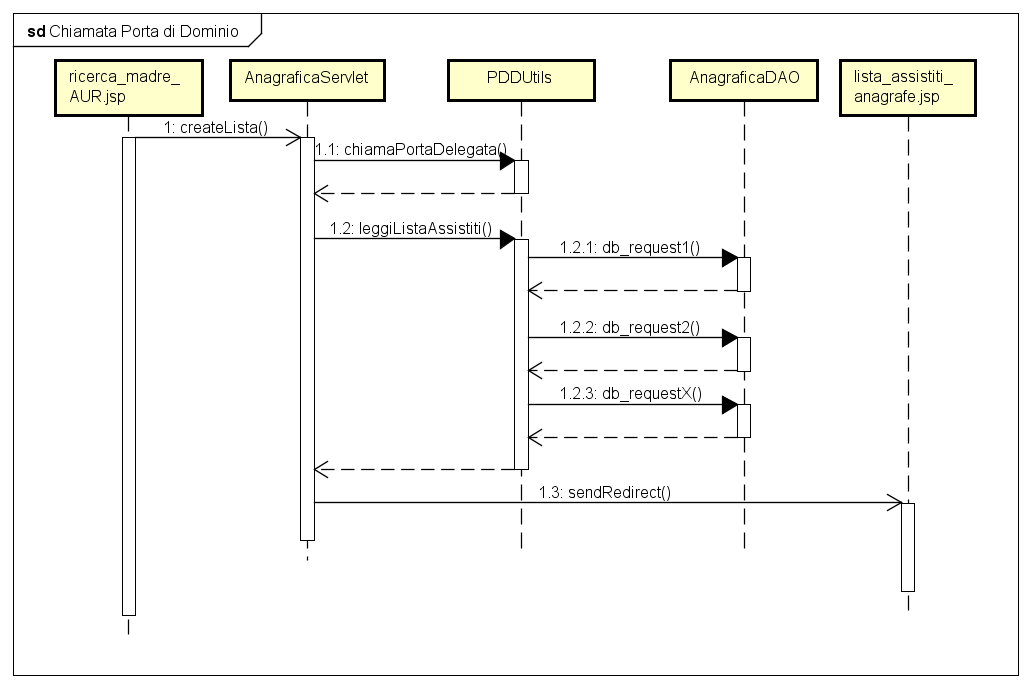
\includegraphics[width=\linewidth]{uml/chiamataportadidominio.png}
	\caption{Diagramma di sequenza - Chiamata alla porta di dominio}
\end{figure}
In questa figura viene descritta la ricerca della madre di un nuovo nato, che può essere facilmente ricondotta anche agli altri due casi di ricerca (padre e paziente).
\\
La chiamata alla porta di dominio dell'\textit{AUR\textsuperscript{\hyperref[sec:gl]{G}}} avviene all'invio della richiesta di ricerca all'applicativo eseguita dalla pagina ricerca\_madre\_AUR.jsp. La richiesta, completa di dati inseriti, viene inoltrata alla servlet AnagraficaServlet tramite il metodo AnagraficaServlet.createLista(). Quest'ultimo scrive i dati in un file xml ed imposta gli altri parametri necessari all'interrogazione dell'\textit{AUR\textsuperscript{\hyperref[sec:gl]{G}}}: l'url ed il metodo di invocazione della porta delegata (classe Costanti.java), e l'intestazione della richiesta (file VisuraAUR\_Intestazione.xml). AnagraficaServlet invoca il metodo PDDUtils.chiamaPortaDelegata() con i parametri sopracitati per fruire del servizio VisureAUR e ne ottiene la risposta. Successivamente invoca PDDUtils.leggiListaAssistiti() fornendo tale risposta come parametro; questo metodo si occupa di interpretare i dati e memorizzarli in un oggetto AnagraficaAssistito. Al termine della chiamata AnagraficaServlet passa, tramite l'oggetto Navigator, alla pagina lista\_assistiti\_anagrafe.jsp la lista dei risultati ottenuti dall'\textit{AUR\textsuperscript{\hyperref[sec:gl]{G}}}, dove verrà organizzata in una tabella facilmente consultabile. Le richieste di accesso al database aziendale sono necessarie per la rielaborazione e l'arricchimento dei dati ottenuti: ad esempio ricavare il comune di residenza a partire dal codice ISTAT ed estrapolarne il distretto sanitario corrispondente.

\subsubsection{AnagraficaServlet}
\begin{figure}[H]
	\centering
	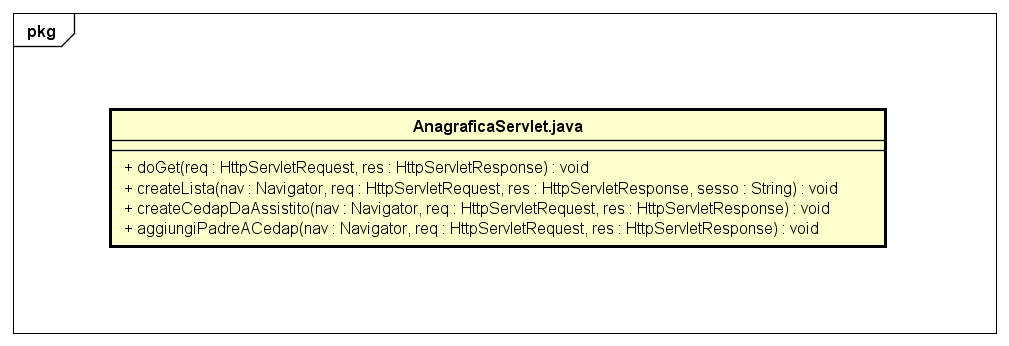
\includegraphics[width=\linewidth]{uml/anagraficaservlet.png}
	\caption{Diagramma di classe - AnagraficaServlet}
\end{figure}
AnagraficaServlet è una servlet Java che si occupa di:
\begin{itemize}
	\item gestire la configurazione dell'interrogazione all'\textit{AUR\textsuperscript{\hyperref[sec:gl]{G}}}, compilando la richiesta (a partire dal file VisuraAUR\_Richiesta.xml) ed inizializzando i parametri della chiamata alla porta di dominio;
    \item creare la lista dei risultati ottenuti dall'\textit{AUR\textsuperscript{\hyperref[sec:gl]{G}}}, reindirizzando alla pagina lista\_assistiti\_anagrafe.jsp che permette di visualizzarli in una tabella facilmente consultabile;
    \item garantire il passaggio di dati indispensabili all'applicativo tramite l'oggetto Navigator quando vengono selezionati una madre, un padre od un paziente dalla lista dei risultati ottenuti dall'\textit{AUR\textsuperscript{\hyperref[sec:gl]{G}}}, reindirizzando alla pagina iniziale corrispondente (madre\_AUR.jsp, padre\_AUR.jsp, paziente.jsp).
\end{itemize}
AnagraficaServlet sfrutta la classe PDDUtils per eseguire la vera e propria chiamata al servizio VisureAUR.

\subsubsection{PazienteServlet e ModificaPazienteLeggi}
PazienteServlet è una servlet Java che si occupa di gestire i dati del paziente dopo aver salvato il suo \textit{certificato di malattia rara\textsuperscript{\hyperref[sec:gl]{G}}} nell'applicativo Malattie Rare.
\\
ModificaPazienteLeggi è una classe contenente metodi di utilità per PazienteServlet. In particolare permette di leggere i dati del paziente immessi, eseguire su di essi i controlli necessari e memorizzarli nel database aziendale assieme al \textit{certificato di malattia rara\textsuperscript{\hyperref[sec:gl]{G}}}. 
\\
Non essendo ancora chiaro come si volesse modificare la procedura di salvataggio dell'IDMPI nel database, ho inserito una mia versione del codice, così da agevolare interventi successivi. Avrei potuto continuare questo lavoro, ma la successiva riorganizzazione del database aziendale avrebbe reso inutile ulteriori modifiche. Questo breve approfondimento è stato molto utile per esplorare la struttura del database e contribuire alla sua rimodellazione.

\subsubsection{PDDUtils}
\begin{figure}[H]
	\centering
	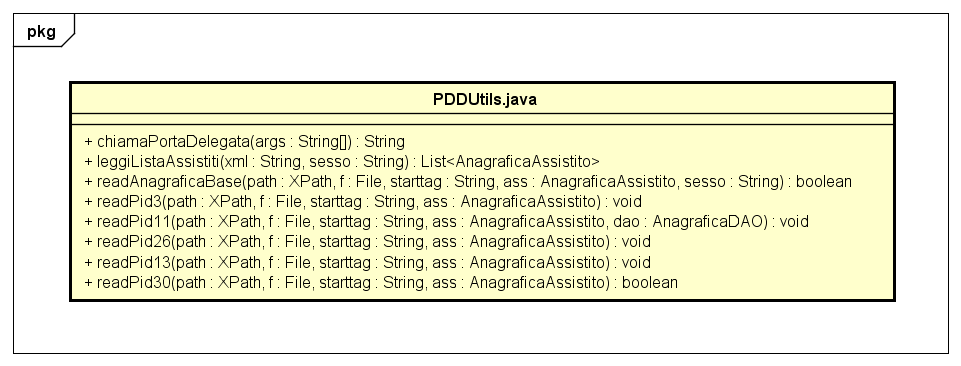
\includegraphics[width=\linewidth]{uml/pddutils.png}
	\caption{Diagramma di classe - PDDUtils}
\end{figure}
PDDUtils è una classe Java contenente metodi di utilità per l'interazione con la porta di dominio dell'\textit{AUR\textsuperscript{\hyperref[sec:gl]{G}}}. In particolare definisce i metodi per l'invio della richiesta e la ricezione, la lettura e la memorizzazione (in un apposito oggetto List<AnagraficaAssistito>) della risposta ottenuta.

\subsubsection{AnagraficaDAO}
\begin{figure}[H]
	\centering
	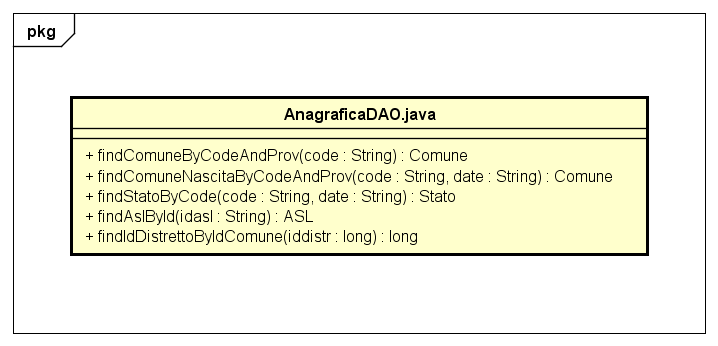
\includegraphics[width=\linewidth]{uml/anagraficadao.png}
	\caption{Diagramma di classe - AnagraficaDAO}
\end{figure}
AnagraficaDAO è una classe Java appartente al design pattern Data Access Object. Contiene metodi per l'accesso al database aziendale che vengono utilizzati per:
\begin{itemize}
    \item eseguire query sul database aziendale, in particolare nella tabelle di scelta dei comuni (per la selezione del luogo di nascita);
    \item aggiungere informazioni ad un oggetto AnagraficaAssistito costruito da un risultato ottenuto dall'\textit{AUR\textsuperscript{\hyperref[sec:gl]{G}}}.
\end{itemize}
Nel primo caso, i metodi di AnagraficaDAO vengono invocati in molteplici punti dell'applicativo, mentre nel secondo caso vengono invocati da PDDUtils.

\subsubsection{Pagine jsp}
Le pagine \textit{jsp\textsuperscript{\hyperref[sec:gl]{G}}} (JavaServer Pages) costituiscono l'interfaccia grafica visibile all'utente, al fine di guidarlo nella navigazione dell'applicativo e fornirgli le informazioni desiderate. Il progetto di stage prevedeva il mio intervento anche nel settore dell'esperienza utente, dunque per rendere accessibili le nuove funzionalità ho creato e modificato alcune pagine \textit{jsp\textsuperscript{\hyperref[sec:gl]{G}}} degli applicativi:
\begin{itemize}
	\item ho creato la pagina ricerca\_madre\_AUR.jsp per permettere la ricerca nell'\textit{AUR\textsuperscript{\hyperref[sec:gl]{G}}} della madre di un nuovo nato;
    \item ho creato la pagina ricerca\_padre\_AUR.jsp per permettere la ricerca nell'\textit{AUR\textsuperscript{\hyperref[sec:gl]{G}}} del padre di un nuovo nato;
    \item ho creato la pagina ricerca\_paziente\_AUR.jsp per permettere la ricerca nell'\textit{AUR\textsuperscript{\hyperref[sec:gl]{G}}} del paziente affetto da malattia rara;
    \item ho creato la pagina lista\_assistiti\_anagrafe.jsp per permettere la visualizzazione dei risultati delal ricerca ottenuti dall'\textit{AUR\textsuperscript{\hyperref[sec:gl]{G}}} e l'evenutale selezione di uno di essi;
    \item ho modificato le pagine madre\_AUR.jsp, padre\_AUR.jsp e paziente.jsp per offrire la funzionalità di ricerca nell'\textit{AUR\textsuperscript{\hyperref[sec:gl]{G}}} ed eseguire molteplici controlli per l'autocompilazione dei campi dati in base alle informazioni ottenute (solo nel caso di un'effettiva ricerca e non di inserimento manuale).
\end{itemize}

\subsubsection{Richiesta al servizio VisureAUR}
La richiesta al servizio VisureAUR deve rispettare alcune regole prestabilite per quanto riguarda la formattazione. Come spiegato precedentemente, la richiesta passa attraverso la porta di dominio dell'azienda e giunge in quella dell'\textit{AUR\textsuperscript{\hyperref[sec:gl]{G}}}. Il messaggio deve essere contenuto in una \textit{busta e-Gov\textsuperscript{\hyperref[sec:gl]{G}}} e rispettare lo standard sanitario \textit{HL7\textsuperscript{\hyperref[sec:gl]{G}}}.
\\
L'intestazione del messaggio è predefinita e viene apposta ad ogni richiesta uscente dalla porta di dominio.
\begin{verbatim}
<Intestazione>
	<Mittente tipo="SPC">*MITTENTE*</Mittente>
	<Destinatario tipo="SPC">*DESTINATARIO*</Destinatario>
	<OraRegistrazione>*DATA ED ORA DI REGISTRAZIONE*</OraRegistrazione>
	<Servizio tipo="SPC">VisureAUR</Servizio>
	<Azione>ricerca</Azione>
	<ProfiloCollaborazione tipo="SPC">EGOV_IT_ServizioSincrono</ProfiloCollaborazione>
	<AllegatoIN>RICHIESTA</AllegatoIN>
	<AllegatoOUT>ECCEZIONE</AllegatoOUT>
	<AllegatoOUT>RISPOSTA</AllegatoOUT>
</Intestazione>
\end{verbatim}
Nell'intestazione sono presenti svariati campi dati, che contengono informazioni sul mittente, sul destinatario, sul messaggio e sull'\textit{accordo di servizio\textsuperscript{\hyperref[sec:gl]{G}}} stipulato. Non sono state necessarie modifiche all'intestazione.
\\
Il messaggio è contenuto nel tag QRY\_A19, predisposto dal \textit{circuito CReSCI\textsuperscript{\hyperref[sec:gl]{G}}} per la ricerca dei dati anagrafici di un assistito. Vi si possono leggere altre informazioni riguardanti le porte di dominio ed il servizio, mentre nel tag QRF che risiedono i dati su cui effettuare la ricerca dell'assistito. Per una consultazione dettagliata della struttura del tag QRY\_A19, consultare la sezione \textit{Appendice\textsuperscript{\hyperref[sec:ap]{A}}} in fondo a questo documento.
\\
La ricerca dell'assistito viene effettuata in base ad alcuni parametri come nome, cognome, data di nascita, codice ISTAT del luogo di nascita, codice fiscale (o codici equivalenti). Questi parametri vengono valorizzati adeguatamente in AnagraficaServlet.

\subsubsection{Note aggiuntive}
Nonostante la maggior parte del lavoro sia stato svolto nelle sezioni precedentemente descritte, sono stati necessari numerosi piccoli accorgimenti in vari luoghi degli applicativi, che per completezza descrivo sinteticamente.
\\
Per permettere agli applicativi di comunicare con l'\textit{AUR\textsuperscript{\hyperref[sec:gl]{G}}}, ho dovuto modificare ed aggiornare i file di configurazione. In particolare ho inserito nel mapping la nuova servlet AnagraficaServlet ed impostato adeguatamente url ed altri parametri della porta delegata dell'azienda.
\\
Per tenere traccia delle nuove informazioni, fornite o necessarie all'\textit{AUR\textsuperscript{\hyperref[sec:gl]{G}}}, sono stati aggiunti campi dati e rispettivi metodi getters e setters alle classi:
\begin{itemize}
	\item AnagraficaAssistito;
	\item Indirizzo;
    \item Comune;
	\item Paziente;
	\item Provincia;
	\item Stato.
\end{itemize}
La struttura delle classi sopracitate rispecchia quella di AnagraficaAssistito, che riporto a scopo esemplificativo.
\begin{figure}[H]
	\centering
	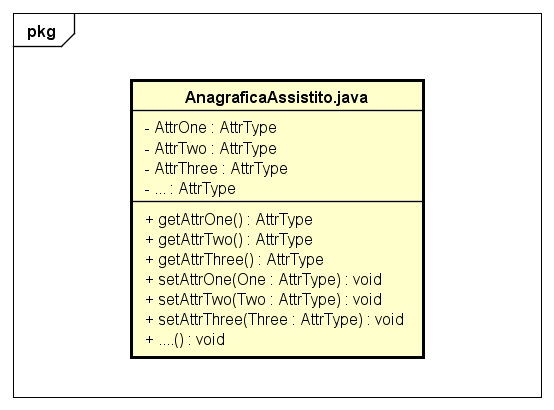
\includegraphics[width=\linewidth]{uml/anagraficaassistito.png}
	\caption{Diagramma di classe - AnagraficaAssistito}
\end{figure}

\noindent Per integrare le nuove funzionalità di ricerca con il precedente control flow, sono state aggiunti alcuni valori al file contenente le costanti globali degli applicativi.
\\
Per generare la lista di scelta dei possibili comuni di nascita ho definito un paio di sql statement, li ho aggiunti alla classe TBL\_\_\_Lookup attraverso la quale vengono invocati ed inclusi la chiamata nella pagina \textit{jsp\textsuperscript{\hyperref[sec:gl]{G}}} di partenza.
\\
Per il corretto funzionamento del nuovo codice, ho recuperato ed inserito le librerie necessarie, sia di Apache Commons che fornite dal \textit{circuito CReSCI\textsuperscript{\hyperref[sec:gl]{G}}} e sviluppate specificamente per le porte di dominio.
\\
Infine ho provveduto a commentare esaustivamente ogni parte di codice da me visionata, come richiesto dall'azienda. Ho descritto lo stato d'entrata e d'uscita di ogni metodo, spiegandone lo scopo. Ad ogni passaggio non banale del codice, ho esplicitato il suo effetto. Nel caso di sezioni particolarmente complesse o da estendere successivamente, ne ho esposto il contesto, la soluzione adottata attualmente ed i suggerimenti per l'eventuale lavoro futuro.

\subsubsection{Esito del lavoro}
Gli obiettivi prefissati sono stati puntualmente conseguiti rispettando le richieste dell'azienda, compresa l'aggiunta di funzionalità e correzioni in seguito ad un'analisi personale del dominio. Non ho riscontrato particolati problematiche, l'unica difficoltà riguardava il codice disordinato, dispersivo e privo di documentazione.

\newpage

\section{ReceiverWS}

\subsection{Richiesta dell'azienda}
Il completamento del lavoro sugli applicativi ha evidenziato alcune lacune nella preparazione per la sottoscrizione del database del \crmr all'\textit{AUR\textsuperscript{\hyperref[sec:gl]{G}}}. La più urgente consisteva nell'istaurare una procedura automatizzata pronta a ricevere aggiornamenti riguardo ai dati degli assistiti (effettuati lato \textit{AUR\textsuperscript{\hyperref[sec:gl]{G}}}). Per soddisfare tale esigenza, l'azienda ha ottenuto dal \textit{circuito CReSCI\textsuperscript{\hyperref[sec:gl]{G}}} un prototipo software per la ricezione degli aggiornamenti tramite il servizio MDB-PLS-WS. Un'ulteriore richiesta è stata quella di documentare approfonditamente tutto ciò che avessi ritenuto rilevante per l'uso e l'estensione di ReceiverWS.

\subsection{Definizione ed analisi degli obiettivi}
Coniugando le potenzialità del prototipo sofware inviatoci e le richieste dell'azienda, ho stabilito gli obiettivi fondamentale che avrebbe dovuto raggiungere ReceiverWS:
\begin{itemize}
	\item creare e configurare il servizio MDB-PLS-WS affinchè comunicasse correttamente con l'\textit{AUR\textsuperscript{\hyperref[sec:gl]{G}}};
	\item configurare il prototipo software affinchè comunicasse correttamente con il servizio MDB-PLS-WS;
    \item salvare gli aggiornamenti ricevuti in un database Oracle, memorizzando il contenuto della \textit{busta e-Gov\textsuperscript{\hyperref[sec:gl]{G}}} in un oggetto di tipo XMLType (che permette query direttamente nei record);
    \item documentare estensivamente le operazioni di configurazione e sviluppo, nonchè fornire esempi di test per la correttezza.
\end{itemize}
La configurazione del servizio MDB-PLS-WS e del prototipo software sono state le parti più impegnative dell'intero stage. La complessità derivava da alcune lacune nella documentazione fornita dal \textit{circuito CReSCI\textsuperscript{\hyperref[sec:gl]{G}}} e dalla scarsa conoscenza della configurazione del sistema interno all'azienda. Dedicando molte ore allo studio di ogni file da modificare e procedendo con cautela, sono comunque riuscito ad ottenere il risultato prestabilito.
\\
La ricezione ed il salvataggio degli aggiornamenti sono stati codificati all'interno di ReceiverWS, seguendo lo scheletro già presente nel prototipo. La conversione degli aggiornamenti ad un oggetto di tipo XMLType è stata realizzata attraverso una procedura a livello del database.

\subsection{Lavoro svolto su ReceiverWS}
Per prima cosa, ho recuperato tutta la documentazione esistente dal sito del \textit{circuito CReSCI\textsuperscript{\hyperref[sec:gl]{G}}}. Quando ho ritenuto di averla studiato abbastanza, ho intrapreso una discussione via email con il referente del \textit{circuito CReSCI\textsuperscript{\hyperref[sec:gl]{G}}}. Quest'ultimo mi ha fornito il prototipo software per la ricezione ed il salvataggio dei dati trasmessi al servizio MDB-PLS-WS. Seguendo le istruzioni descritte, ho tentato di far funzionare il prototipo ma senza successo. Nel mentre sono stato ricontattato dal referente, che mi ha informato di un suo errore: il prototipo faceva riferimento alla versione 1.0 delle porte di dominio, mentre quella attuale era la 1.1. A quel punto ho notato che la documentazione stessa si basava sulla versione 1.0 delle porte di dominio, risultando dunque obsoleta. Non conoscendo le differenze tra tali versioni, non ho potuto affidarmi completamente alla documentazione esistente. A volte, quando la logica o l'esperienza sono bastavano, ho dovuto purtroppo procedere per tentativi.
\\
All'avvenuta ricezione di un secondo modello di prototipo ho potuto iniziare a lavorare a pieno regime su ReceiverWS. Dopo aver analizzato il nuovo codice, ho apportato le opportune modifiche: in particolare il collegamento al database Oracle del \crmr. Una volta ultimati i cambiamenti, ho compresso il tutto in un archivio jar affinchè potessi installarlo nella porta di dominio aziendale.
\\
La porta di dominio del \crmr è stata installata all'interno del loro webserver Apache Tomcat. La porta di dominio, il webserver Apache Tomcat ed il database Oracle aziendali hanno subito numerosi intervenuti nel corso delle attività di configurazione, che si possono riassumere nei seguenti punti:
\begin{itemize}
	\item installazione dei driver per il database;
	\item installazione delle librerie;
    \item installazione di altri file;
    \item modifiche ai file di configurazione.
\end{itemize}
Le sopracitate attività di configurazione sono state eseguite attraverso il software WinSCP e rigorosamente all'interno dell'ambiente di test.

\subsubsection{Installazione dei driver per il database}
Per la comunicazione tra Apache Tomcat ed il database Oracle ho installato il driver \textit{ojdbc14.jar} (non era abbastanza aggiornato per la versione \textit{ojdbc6}).

\subsubsection{Installazione delle librerie}
Le librerie \textit{CorePDD} sono fondamentali per il funzionamento della porta di dominio. Il loro download si trovava nella sezione apposita del sito del \textit{circuito CReSCI\textsuperscript{\hyperref[sec:gl]{G}}}. Ho provveduto dunque alla loro installazione all'interno di Apache Tomcat, assieme all'installazione del file \textit{ReceiverWS.jar} che regola la lettura, l'elaborazione ed il salvataggio nel database dei messaggi ricevuti attraverso il servizio MDB-PLS-WS. Inoltre ho aggiunto il file \textit{Portadidominio.xml} alla cartella di configurazione di Catalina affinchè regoli la connessione con il database Oracle.

\subsubsection{Installazione di altri file}
Ho aggiunto i seguenti file a varie sottocartelle appartenenti alla porta di dominio:
\begin{itemize}
	\item \textit{Ack.xml} contenente la struttura del messaggio di acknowledgement;
    \item \textit{Sissr-anagrafe-receiver.properties} contenente i dati per la connessione al database Oracle e vari path locali;
    \item \textit{Web.xml} contenente il riferimento alla risorsa \textit{driver JDBC}.
\end{itemize}

\subsubsection{Modifiche ai file di configurazione}
L'individuazione dei file per configurare la comunicazione della porta di dominio aziendale con il servizio MDB-PLS-WS è stata l'attività più complessa ed articolata. La documentazione presentava affermazioni discordanti ed il colloquio telefonico con il referente del prototipo riguardo a queste perplessità è sfociato in soluzioni completamente differenti. Queste problematiche si sono unite alla totale mancanza di direttive riguardanti la struttura di Apache Tomcat. Sono così stato costretto ad investire numerose ore nello studio della situazione esistente, altrimenti non avrei potuto agire senza rischiare gravi conseguenze.
\\
Il software \textit{XMLdbGUI} fornisce un'interfaccia client per la gestione dei database XML. Essendo consigliato dal \textit{circuito CReSCI\textsuperscript{\hyperref[sec:gl]{G}}} ne ho fatto uso per le attività sui seguenti file:
\begin{itemize}
	    \item in \textit{RegistroServizi.xml}, contenente l'elenco dei servizi della porta di dominio, ho inserito il nuovo servizio MDB-PLS-WS;
	\item in \textit{Servizi.wsdd}, contenente l'elenco dei parametri IN/OUT dei servizi della porta di dominio, ho inserito i parametri del nuovo servizio MDB-PLS-WS;
    \item in\textit{PAWebServiceWrapper.xml}, contenente l'elenco dei wevservices (la cui implementazione come servizi è definita in \textit{Servizi.wsdd}), ho inserito il webservice MDB-PLS-WS.
\end{itemize}
Successivamente ho svolto le seguenti operazioni aggiuntive:
\begin{itemize}
	\item ho creato il file \textit{CtxServizioMDB-PLS-WS.xml} contenente la definizione dei parametri e del workflow del servizio MDB-PLS-WS;
    \item nel file \textit{Server-config.wsdd}, contenente i servizi esposti dal server, ho inserito il servizio WebServiceReceiver;
    \item nel file \textit{Log4j.xml}, contenente le impostazioni per il logging della porta di dominio, ho inserito l'appender TracciaReceiverCEDAP ed il relativo logger.
\end{itemize}
Al termine del lavoro su ReceiverCEDAP, il software ed il servizio MDB-PLS-WS erano correttamente configurati mentre le informazioni trasmesse a tale servizio venivano puntualmente salvate nel database Oracle. Inoltre la documentazione è stata redatta con un livello di dettaglio adeguato alle richieste dell'azienda.

\newpage

\section{SenderWS}

\subsection{Richiesta dell'azienda}
La richiesta dell'azienda consisteva nello sviluppare un software esemplificativo, tramite qualsiasi tipo di implementazione, che permettesse di inviare messaggi al servizio MDB-PLS-WS (che funge da canale di comunicazione per le informazioni su qualsiasi assistito della Regione Veneto). SenderWS vuole essere una base per l'implementazione di una procedura automatizzata d'invio delle esenzioni (garantite dal \textit{certificato di malattia rara\textsuperscript{\hyperref[sec:gl]{G}}}) tramite la porta di dominio aziendale. 

\subsection{Definizione ed analisi degli obiettivi}
Prima di definire gli obiettivi di SenderWS, ho analizzato il contesto in cui avrei dovuto operare, in quanto presentava diverse problematiche:
\begin{itemize}
	\item SenderWS avrebbe dovuto comunicare con il \textit{circuito CReSCI\textsuperscript{\hyperref[sec:gl]{G}}}, ma non era stato ancora stabilito alcun \textit{accordo di servizio\textsuperscript{\hyperref[sec:gl]{G}}};
    \item SenderWS avrebbe dovuto essere un software a scopo esemplificativo capace solo di poche funzioni di base da estendere in futuro;
    \item SenderWS non avrebbe dovuto essere vincolato dalla propria implementazione attuale, in quanto non era stato deciso se in futuro sarebbe stato integrato negli applicativi oppure sarebbe stato un software autonomo.
\end{itemize}
Riguardo alla prima problematica, ho fatto in modo che SenderWS trasmettesse il proprio messaggio al servizio MDB-PLS-WS al posto del fantomatico futuro servizio. In questo modo il messaggio viene inviato a noi stessi e viene opportunamente ricevuto da ReceiverWS. Purtroppo non c'era altro modo di testarne la corretta esecuzione, vista la mancanza di un servizio apposito. Comunque cambiare successivamente il servizio di trasmissione del messaggio si tratta di un procedimento rapido ed indolore.
\\
Le altre due problematiche sono state risolte con l'implementazione di SenderWS come webservice. Le motivazioni sono state:
\begin{itemize}
	\item concludere uno stage sui webservices sviluppando un software che ne faccia uso è un passo estremamente logico;
    \item l'interoperabilità, la componibilità ed il disaccoppiamento dal sistema di deployment garantite dai webservices sono proprietà fondamentali quando non si possiedono le specifiche del sistema stesso.
\end{itemize}

\subsection{Lavoro svolto su SenderWS}
Perla creazione del webservice SenderWS ho sfruttato la Web Tools Platform (WTP) di Eclipse, che fornisce automaticamente il client per testarlo.
\\
SenderWS espone due operazioni:
\begin{itemize}
	\item \textbf{addToQueue(String,String,String)(void)} aggiunge alla coda di invio le informazioni inserite nell'input;
    \item \textbf{sendUpdates(void)(void)} invia il primo oggetto presente nella coda.
\end{itemize}
Segue una breve descrizione dei package presenti in SenderWS:
\begin{itemize}
	\item it.cedap.anagrafe.WebServiceSender espone le proprie operazioni all'esterno;
    \item it.cedap.anagrafe.Sender definisce la business logic;
    \item it.cedap.anagrafe.Data descrive le strutture dati degli oggetti;
    \item it.cedap.anagrafe.PDD definisce le classi e gli oggetti necessari all'utilizzo della porta di dominio;
	\item it.cedap.anagrafe.Utils contiene le utilità (conversioni tra stringhe e documenti xml).
\end{itemize}
Il codice è stato opportunamente corredato da commenti ed include una semplice gestione delle eccezioni.

\newpage

\section{Considerazioni finali}

\subsection{Sviluppi futuri dei software}
Gli applicativi CEDAP e Malattie Rare sono in continua evoluzione, in quanto le necessità degli utenti ed i cambiamenti alla legislazione mutano rapidamente. Sono fiducioso però che l'integrazione con l'\textit{AUR\textsuperscript{\hyperref[sec:gl]{G}}} aumenterà di importanza nel futuro e potrà essere estesa per assolvere una vasta gamma di compiti.
\\
Già da alcuni anni l'Europa preme per diffondere il concetto di e-Government e potenziare i circuiti di interoperabilità tra entità pubbliche. Sincronizzare i dati anagrafici dei database locali il database centralizzato dell'\textit{AUR\textsuperscript{\hyperref[sec:gl]{G}}} comporterà un grande miglioramento del sistema sanitario. Ad oggi, non esiste un metodo rapido per rintracciare correttamente la storia clinica delle persone. Questo bisogno di informazioni è emerso già durante il periodo di stage: infatti mi è stato chiesto più di una volta di controllare i dati anagrafici di un particolare assistito.
\\
I webservices offerti dalla Regione Veneto verranno certamente ampliati e perfezionati: possedere la capacità di sfruttarli beneficia sia l'azienda che gli abitanti della Regione Veneto.
\\
Dal lato opposto anche esporre i propri webservices può portare notevoli vantaggi. Attualmente, le esenzioni ottenute dal \textit{certificato di malattia rara\textsuperscript{\hyperref[sec:gl]{G}}} vengono inviate tramite una procedura batch. Tale modalità operativa è dispendiosa in quanto soggetta ad errori umani e non permette una sincronizzazione speculare delle informazioni.
\\
Ritengo sia fondamentale un ulteriore sviluppo dei software ReceiverWS e SenderWS, che offrono funzionalità ancora limitate rispetto alle loro potenzialità. La gestione delle informazioni dei pazienti è estremamente onerosa per il \crmr e richiede costanti attenzioni ad ogni nuovo rilascio. Automatizzare i canali di entrata ed uscita di tali informazioni alleggerirebbe in modo significativo questo carico.

\subsection{Esperienza acquisita}
Lavorare al \crmr mi ha permesso di approcciarmi concretamente con molteplici argomenti trattati durante il percorso di studi di laurea triennale in Informatica.
\\
Lo stage ha comportato un confronto quotidiano con le richieste di varie figure lavorative (medici, farmacisti, statistici), spesso prive di conoscenze tecniche informatiche. Durante questo periodo ho migliorato le mie capacità di comunicazione e di esposizione di situazioni complesse ad un pubblico poco esperto. Valuto questa un'abilità fondamentale nel mondo del lavoro in quanto spesso è necessario fornire spiegazioni semplici ma efficaci, indipendentemente dal livello di conoscenze degli ascoltatori.
\\
Lo studio e l'utilizzo delle porte di dominio è stato particolarmente formativo. Le tematiche di e-Government e di interoperabilità sono estremamente attuali e potranno solo acquisire maggior importanza nel futuro. Conoscerne i meccanismi ed i circuiti è certamente un vantaggio vista l'ampio settore in cui vengono impiegati. Di ancor più ampio respiro è il tema dei webservices ormai onnipresenti nel mondo dell'informatica.
\\
In definitiva, ritengo lo stage da me condotto un'esperienza preziosa che mi ha arricchito di conoscenze utili per la mia formazione professionale e personale.


\newpage

\vspace*{\fill}

\newpage

\section{Appendice}
\label{sec:ap}

\subsection{Analisi dei requisiti}

\subsubsection{Casi d'uso}
Gli ambiti dei casi d'uso si possono dividere in tre flussi operativi:
\begin{itemize}
	\item ricerca ed inserimento della madre del nuovo nato nell'applicativo CEDAP;
    \item ricerca ed inserimento del padre del nuovo nato nell'applicativo CEDAP;
    \item ricerca ed inserimento del paziente affetto da malattia rara nell'applicativo Malattie Rare.
\end{itemize} 
Le differenze tra questi ambiti tuttavia sono minime, infatti la ricerca viene effettuata con le stesse modalità tramite il servizio VisureAUR. Inoltre, i dati anagrafici fondamentali richiesti per la compilazione dei certificati sono i medesimi per madre, padre e paziente.
\\
Verranno dunque trattati in dettaglio solo i casi d'uso per la procedura di ricerca ed inserimento della madre del nuovo nato nell'applicativo CEDAP.
\\
Ritengo inoltre che l'esposizione del progetto non richieda approfondimenti estremi riguardo ai casi d'uso presentati ed il grado di dettaglio qui raggiunto sia sufficiente. 

\subsubsubsection{Registrazione nuovo CEDAP}

\begin{figure}[H]
	\centering
	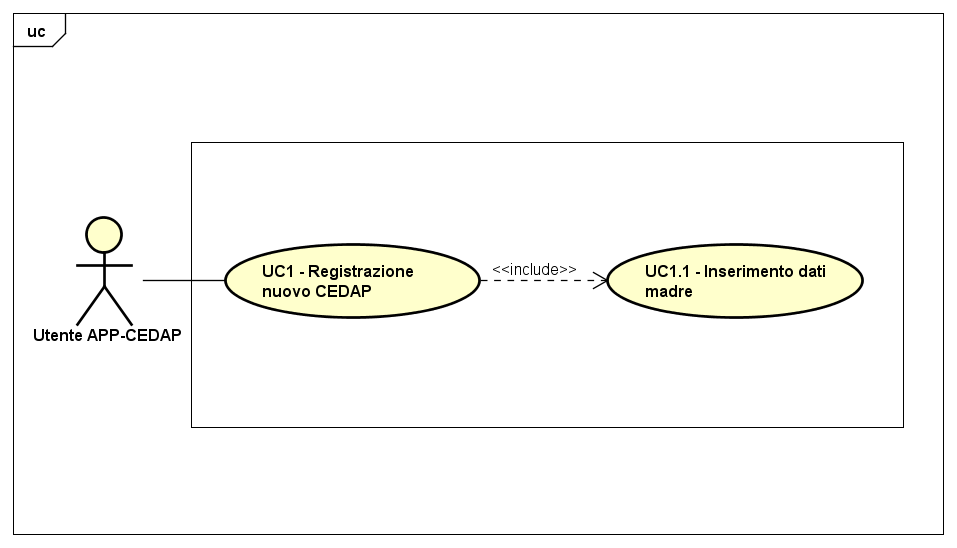
\includegraphics[width=\linewidth]{uml/UC1.png}
    \label{fig:UC1}
	\caption{UC1 - Registrazione nuovo CEDAP}
\end{figure}

\subsubsubsection{Caso d'uso UC1: Registrazione nuovo CEDAP}
\label{UC1}

\textbf{Attori principali}: Utente APP-CEDAP.
\\
\textbf{Attori secondari}: AUR.
\\
\textbf{Descrizione}: L'attore registra un nuovo CEDAP nell'applicativo CEDAP.
\\
\textbf{Pre-condizioni}: L'attore è autenticato all'applicativo CEDAP.
\\
\textbf{Post-condizioni}: L'attore ha registrato un nuovo CEDAP nell'applicativo CEDAP, dopo aver compilato i campi obbligatori delle sezioni del nuovo CEDAP.
\\
\textbf{Scenario principale}: L'attore può registrare un nuovo CEDAP nell'applicativo CEDAP (UC1), venendo reindirizzato alla sezione madre del nuovo CEDAP (UC1.1).

\begin{figure}[H]
	\centering
	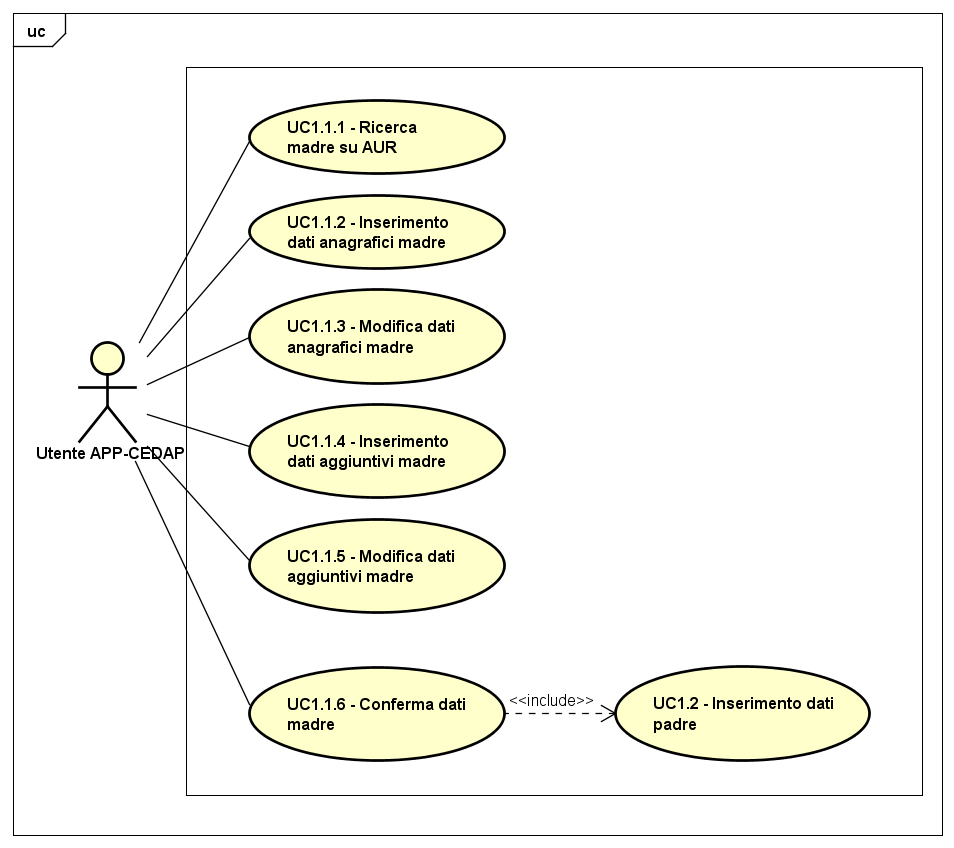
\includegraphics[width=\linewidth]{uml/UC1_1.png}
    \label{fig:UC1.1}
	\caption{UC1.1 - Inserimento dati madre}
\end{figure}

\subsubsubsection{Caso d'uso UC1.1: Inserimento dati madre}
\label{UC1.1}

\textbf{Attori principali}: Utente APP-CEDAP.
\\
\textbf{Attori secondari}: AUR.
\\
\textbf{Descrizione}: L'attore inserisce i dati della madre relativa al nuovo CEDAP nell'applicativo CEDAP.
\\
\textbf{Pre-condizioni}: L'attore ha scelto di effettuare la registrazione di nuovo CEDAP nell'applicativo CEDAP.
\\
\textbf{Post-condizioni}: L'attore ha inserito i dati della madre relativa al nuovo CEDAP nell'applicativo CEDAP.
\\
\textbf{Scenario principale}: L'attore può inserire i dati della madre relativa al nuovo CEDAP nell'applicativo CEDAP (UC1.1).

\begin{figure}[H]
	\centering
	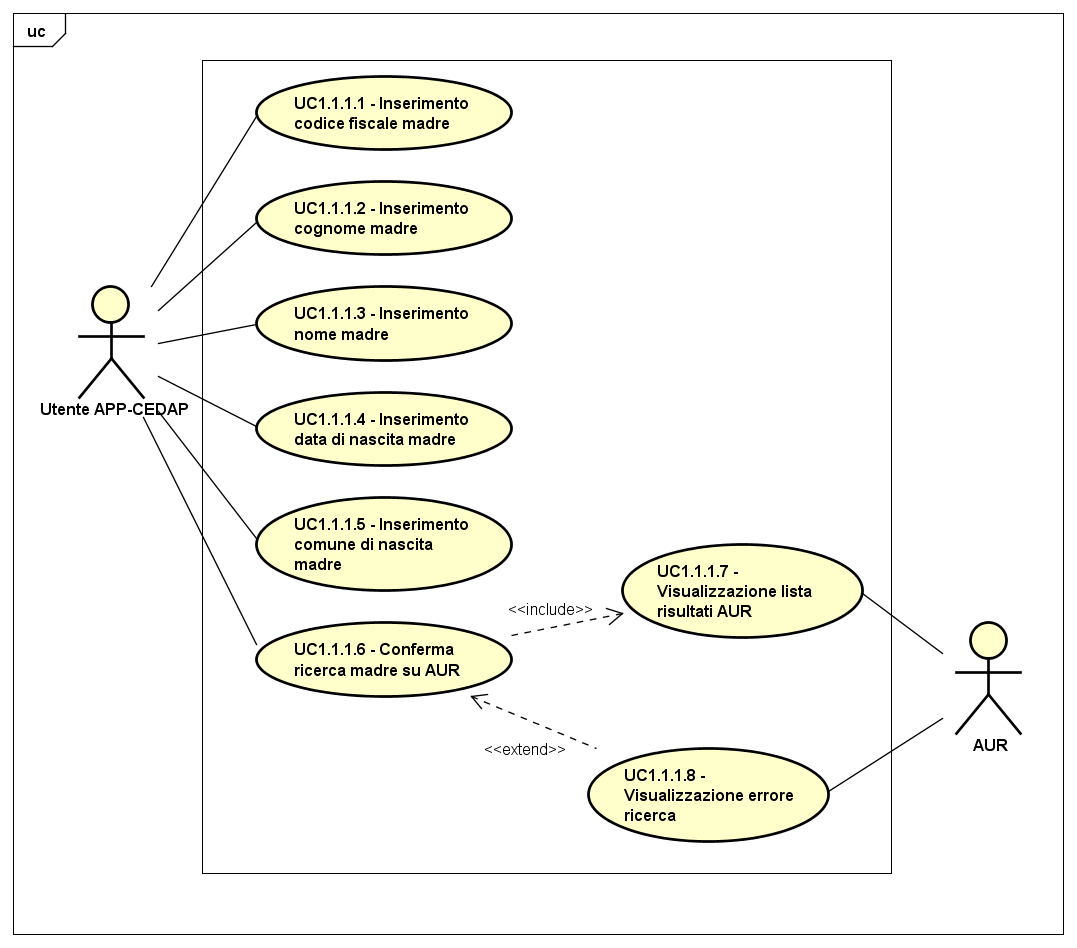
\includegraphics[width=\linewidth]{uml/UC1_1_1.png}
    \label{fig:UC1.1.1}
	\caption{UC1.1.1 - Ricerca dati madre su AUR}
\end{figure}

\subsubsubsection{Caso d'uso UC1.1.1: Ricerca dati madre su AUR}
\label{UC1.1.1}

\textbf{Attori principali}: Utente APP-CEDAP.
\\
\textbf{Attori secondari}: AUR.
\\
\textbf{Descrizione}: L'attore ricerca i dati della madre nell'AUR attraverso l'applicativo CEDAP.
\\
\textbf{Pre-condizioni}: L'attore ha scelto di effettuare la registrazione di nuovo CEDAP nell'applicativo CEDAP.
\\
\textbf{Post-condizioni}: L'attore ha ricercato i dati della madre nell'AUR attraverso l'applicativo CEDAP.
\\
\textbf{Scenario principale}: L'attore ricerca i dati della madre nell'AUR attraverso l'applicativo CEDAP (UC1.1.1).


\subsubsubsection{Caso d'uso UC1.1.1.1 fino ad UC1.1.1.5: Inserimento dati ricerca madre}
\label{UC1.1.1.15}

\textbf{Attori principali}: Utente APP-CEDAP.
\\
\textbf{Descrizione}: L'attore inserisce i dati di ricerca della madre nell'applicativo CEDAP.
\\
\textbf{Pre-condizioni}: L'attore ha scelto di effettuare la ricerca della madre nell'AUR attraverso l'applicativo CEDAP.
\\
\textbf{Post-condizioni}: L'attore ha inserito i dati di ricerca della madre nell'applicativo CEDAP.
\\
\textbf{Scenario principale}: L'attore può inserire ii dati di ricerca della madre nell'applicativo CEDAP.


\subsubsubsection{Caso d'uso UC1.1.1.6: Conferma ricerca madre su AUR}
\label{UC1.1.1.6}

\textbf{Attori principali}: Utente APP-CEDAP.
\\
\textbf{Descrizione}: L'attore conferma la ricerca dei dati della madre sull'AUR attraverso l'applicativo CEDAP.
\\
\textbf{Pre-condizioni}: L'attore ha scelto di effettuare la ricerca della madre nell'AUR attraverso l'applicativo CEDAP.
\\
\textbf{Post-condizioni}: L'attore ha confermato la ricerca dei dati della madre sull'AUR attraverso l'applicativo CEDAP e viene reindirizzato alla visualizzazione dei risultati ottenuti.
\\
\textbf{Scenario principale}: L'attore può confermare la ricerca dei dati della madre sull'AUR attraverso l'applicativo CEDAP (UC1.1.1.6), venendo reindirizzato alla visualizzazione dei risultati ottenuti (UC1.1.1.7).
\\
\textbf{Scenari alternativi}: L'attore visualizza un messaggio di errore nel caso gli inserimenti siano errati (es. codice fiscale non valido, formato della data non valido) (UC1.1.1.8).


\subsubsubsection{Caso d'uso UC1.1.1.7: Visualizzazione lista risultati AUR}
\label{UC1.1.1.7}

\textbf{Attori principali}: Utente APP-CEDAP.
\\
\textbf{Attori secondari}: AUR.
\\
\textbf{Descrizione}: L'attore visualizza la lista dei risultati ottenuti dalla ricerca sull'AUR attraverso l'applicativo CEDAP.
\\
\textbf{Pre-condizioni}: L'attore ha scelto di effettuare la ricerca della madre nell'AUR attraverso l'applicativo CEDAP.
\\
\textbf{Post-condizioni}: L'attore ha visualizzato la lista dei risultati ottenuti dalla ricerca sull'AUR attraverso l'applicativo CEDAP.
\\
\textbf{Scenario principale}: L'attore può visualizzare la lista dei risultati ottenuti dalla ricerca sull'AUR attraverso l'applicativo CEDAP (UC1.1.1.7).


\subsubsubsection{Caso d'uso UC1.1.1.8: Visualizzazione errore ricerca}
\label{UC1.1.1.8}

\textbf{Attori principali}: Utente APP-CEDAP.
\\
\textbf{Attori secondari}: AUR.
\\
\textbf{Descrizione}: L'attore visualizza l'errore sui parametri di ricerca nell'applicativo CEDAP.
\\
\textbf{Pre-condizioni}: L'attore ha scelto di effettuare la ricerca della madre nell'AUR attraverso l'applicativo CEDAP.
\\
\textbf{Post-condizioni}: L'attore ha visualizzato l'errore sui parametri di ricerca nell'applicativo CEDAP.
\\
\textbf{Scenario principale}: L'attore può visualizzare l'errore sui parametri di ricerca nell'applicativo CEDAP (UC1.1.1.8).



\subsubsubsection{Caso d'uso UC1.1.2: Inserimento dati anagrafici madre}
\label{UC1.1.2}

\textbf{Attori principali}: Utente APP-CEDAP.
\\
\textbf{Attori secondari}: AUR.
\\
\textbf{Descrizione}: L'attore inserisce i dati anagrafici della madre relativa al nuovo CEDAP nell'applicativo CEDAP.
\\
\textbf{Pre-condizioni}: L'attore ha scelto di effettuare la registrazione di nuovo CEDAP nell'applicativo CEDAP.
\\
\textbf{Post-condizioni}: L'attore ha inserito i dati anagrafici della madre relativa al nuovo CEDAP nell'applicativo CEDAP.
\\
\textbf{Scenario principale}: L'attore può inserire i dati anagrafici della madre relativa al nuovo CEDAP nell'applicativo CEDAP (UC1.1.2).

\subsubsubsection{Caso d'uso UC1.1.3: Modifica dati anagrafici madre}
\label{UC1.1.3}

\textbf{Attori principali}: Utente APP-CEDAP.
\\
\textbf{Attori secondari}: AUR.
\\
\textbf{Descrizione}: L'attore modifica i dati anagrafici della madre relativa al nuovo CEDAP nell'applicativo CEDAP.
\\
\textbf{Pre-condizioni}: L'attore ha scelto di effettuare la registrazione di nuovo CEDAP nell'applicativo CEDAP.
\\
\textbf{Post-condizioni}: L'attore ha modificato i dati anagrafici della madre relativa al nuovo CEDAP nell'applicativo CEDAP.
\\
\textbf{Scenario principale}: L'attore può modificare i dati anagrafici della madre relativa al nuovo CEDAP nell'applicativo CEDAP (UC1.1.3).


\subsubsubsection{Caso d'uso UC1.1.4: Inserimento dati aggiuntivi madre}
\label{UC1.1.4}

\textbf{Attori principali}: Utente APP-CEDAP.
\\
\textbf{Attori secondari}: AUR.
\\
\textbf{Descrizione}: L'attore inserisce i dati aggiuntivi della madre relativa al nuovo CEDAP nell'applicativo CEDAP.
\\
\textbf{Pre-condizioni}: L'attore ha scelto di effettuare la registrazione di nuovo CEDAP nell'applicativo CEDAP.
\\
\textbf{Post-condizioni}: L'attore ha inserito i dati aggiuntivi della madre relativa al nuovo CEDAP nell'applicativo CEDAP.
\\
\textbf{Scenario principale}: L'attore può inserire i dati aggiuntivi della madre relativa al nuovo CEDAP nell'applicativo CEDAP (UC1.1.4).


\subsubsubsection{Caso d'uso UC1.1.5: Modifica dati aggiuntivi madre}
\label{UC1.1.5}

\textbf{Attori principali}: Utente APP-CEDAP.
\\
\textbf{Attori secondari}: AUR.
\\
\textbf{Descrizione}: L'attore modifica i dati aggiuntivi della madre relativa al nuovo CEDAP nell'applicativo CEDAP.
\\
\textbf{Pre-condizioni}: L'attore ha scelto di effettuare la registrazione di nuovo CEDAP nell'applicativo CEDAP.
\\
\textbf{Post-condizioni}: L'attore ha modificato i dati aggiuntivi della madre relativa al nuovo CEDAP nell'applicativo CEDAP.
\\
\textbf{Scenario principale}: L'attore può modificare i dati aggiuntivi della madre relativa al nuovo CEDAP nell'applicativo CEDAP (UC1.1.5).


\subsubsubsection{Caso d'uso UC1.1.6: Conferma dati madre}
\label{UC1.1.6}

\textbf{Attori principali}: Utente APP-CEDAP.
\\
\textbf{Attori secondari}: AUR.
\\
\textbf{Descrizione}: L'attore conferma i dati della madre relativa al nuovo CEDAP nell'applicativo CEDAP.
\\
\textbf{Pre-condizioni}: L'attore ha scelto di effettuare la registrazione di nuovo CEDAP nell'applicativo CEDAP.
\\
\textbf{Post-condizioni}: L'attore ha confermato i dati della madre relativa al nuovo CEDAP nell'applicativo CEDAP.
\\
\textbf{Scenario principale}: L'attore può confermare i dati della madre relativa al nuovo CEDAP nell'applicativo CEDAP (UC1.1.6), venendo reindirizzato all'inserimento dei dati del padre relativo al nuovo CEDAP (UC1.2).


\subsubsubsection{Caso d'uso UC1.2: Inserimento dati padre}
\label{UC1.2}

\textbf{Attori principali}: Utente APP-CEDAP.
\\
\textbf{Attori secondari}: AUR.
\\
\textbf{Descrizione}: L'attore inserisce i dati del padre relativo al nuovo CEDAP nell'applicativo CEDAP.
\\
\textbf{Pre-condizioni}: L'attore ha scelto di effettuare la registrazione di nuovo CEDAP nell'applicativo CEDAP ed ha compilato i campi obbligatori della sezione madre.
\\
\textbf{Post-condizioni}: L'attore ha inserito i dati del padre relativo al nuovo CEDAP nell'applicativo CEDAP.
\\
\textbf{Scenario principale}: L'attore inserisce i dati del padre relativo al nuovo CEDAP nell'applicativo CEDAP.
\\
\textbf{Scenari alternativi}: L'attore visualizza un messaggio di errore nel caso l'inserimento sia fallito (Es: dati non corretti, problemi di connessione).


\subsubsubsection{Caso d'uso UC1.3: Inserimento dati gravidanza}
\label{UC1.3}

\textbf{Attori principali}: Utente APP-CEDAP.
\\
\textbf{Attori secondari}: AUR.
\\
\textbf{Descrizione}: L'attore inserisce i dati della gravidanza relativa al nuovo CEDAP nell'applicativo CEDAP.
\\
\textbf{Pre-condizioni}: L'attore ha scelto di effettuare la registrazione di nuovo CEDAP nell'applicativo CEDAP ed ha compilato i campi obbligatori delle sezioni madre e padre.
\\
\textbf{Post-condizioni}: L'attore ha inserito i dati della gravidanza relativa al nuovo CEDAP nell'applicativo CEDAP.
\\
\textbf{Scenario principale}: L'attore inserisce i dati della gravidanza relativa al nuovo CEDAP nell'applicativo CEDAP.
\\
\textbf{Scenari alternativi}: L'attore visualizza un messaggio di errore nel caso l'inserimento sia fallito (Es: dati non corretti, problemi di connessione).


\subsubsubsection{Caso d'uso UC1.4: Inserimento dati parto}
\label{UC1.4}

\textbf{Attori principali}: Utente APP-CEDAP.
\\
\textbf{Attori secondari}: AUR.
\\
\textbf{Descrizione}: L'attore inserisce i dati del parto relativo al nuovo CEDAP nell'applicativo CEDAP.
\\
\textbf{Pre-condizioni}:  L'attore ha scelto di effettuare la registrazione di nuovo CEDAP nell'applicativo CEDAP ed ha compilato i campi obbligatori delle sezioni madre, padre e gravidanza.
\\
\textbf{Post-condizioni}: L'attore ha inserito i dati del parto  relativo al nuovo CEDAP nell'applicativo CEDAP.
\\
\textbf{Scenario principale}: L'attore inserisce i dati del parto relativo al nuovo CEDAP nell'applicativo CEDAP.
\\
\textbf{Scenari alternativi}: L'attore visualizza un messaggio di errore nel caso l'inserimento sia fallito (Es: dati non corretti, problemi di connessione).


\subsubsection{Requisiti}

\subsubsubsection{Tabella dei requisiti APP-CEDAP}

\begin{longtable}{|l|p{10cm}|}

\hline \multicolumn{1}{|c|}{\textbf{Requisito}} & \multicolumn{1}{c|}{\textbf{Descrizione}} \\ \hline 
\endfirsthead

\multicolumn{2}{c}%
{{\bfseries \tablename\ \thetable{} -- continua dalla pagina precedente}} \\
\hline \multicolumn{1}{|c|}{\textbf{Requisito}} & \multicolumn{1}{c|}{\textbf{Descrizione}} \\ \hline 
\endhead

\hline \multicolumn{2}{|r|}{{Continua nella pagina successiva}} \\ \hline
\endfoot

\hline \hline
\endlastfoot

OF1 & L'utente può inserire un nuovo CEDAP in APP-CEDAP \\

OF1.1 & L'utente può inserire i dati della madre del nuovo CEDAP in APP-CEDAP \\

OF1.1.1 & L'utente può ricercare la madre del nuovo CEDAP nell'AUR tramite APP-CEDAP \\

OF1.1.1.1 & L'utente può inserire il codice fiscale della madre del nuovo CEDAP per la ricerca nell'AUR tramite APP-CEDAP \\
OF1.1.1.2 & L'utente può inserire il cognome della madre del nuovo CEDAP per la ricerca nell'AUR tramite APP-CEDAP \\
OF1.1.1.3 & L'utente può inserire il nome della madre del nuovo CEDAP per la ricerca nell'AUR tramite APP-CEDAP \\
OF1.1.1.4 & L'utente può inserire la data di nascita della madre del nuovo CEDAP per la ricerca nell'AUR tramite APP-CEDAP \\
OF1.1.1.5 & L'utente può inserire il comune di nascita della madre del nuovo CEDAP per la ricerca nell'AUR tramite APP-CEDAP \\
OF1.1.1.6 & L'utente può confermare la ricerca della madre del nuovo CEDAP nell'AUR tramite APP-CEDAP \\
OF1.1.1.7 & L'utente può visualizzare la lista dei risultati ottenuti dalla ricerca della madre nell'AUR tramite APP-CEDAP \\
OF1.1.1.8 & L'utente può visualizzare un messaggio di errore riguardante la ricerca della madre nell'AUR tramite APP-CEDAP \\

OF1.1.2 & L'utente può inserire i dati anagrafici della madre del nuovo CEDAP in APP-CEDAP \\
OF1.1.3 & L'utente può modificare i dati anagrafici della madre del nuovo CEDAP in APP-CEDAP \\
OF1.1.4 & L'utente può inserire i dati aggiuntivi della madre del nuovo CEDAP in APP-CEDAP \\
OF1.1.5 & L'utente può modificare i dati aggiuntivi della madre del nuovo CEDAP in APP-CEDAP \\
OF1.1.6 & L'utente può confermare i dati della madre del nuovo CEDAP immessi in APP-CEDAP \\

OF1.2 & L'utente può inserire i dati del padre del nuovo CEDAP in APP-CEDAP \\

OF1.2.1 & L'utente può ricercare il padre del nuovo CEDAP nell'AUR tramite APP-CEDAP \\

OF1.2.1.1 & L'utente può inserire il codice fiscale del padre del nuovo CEDAP per la ricerca nell'AUR tramite APP-CEDAP \\
OF1.2.1.2 & L'utente può inserire il cognome del padre del nuovo CEDAP per la ricerca nell'AUR tramite APP-CEDAP \\
OF1.2.1.3 & L'utente può inserire il nome del padre del nuovo CEDAP per la ricerca nell'AUR tramite APP-CEDAP \\
OF1.2.1.4 & L'utente può inserire la data di nascita del padre del nuovo CEDAP per la ricerca nell'AUR tramite APP-CEDAP \\
OF1.2.1.5 & L'utente può inserire il comune di nascita del padre del nuovo CEDAP per la ricerca nell'AUR tramite APP-CEDAP \\
OF1.2.1.6 & L'utente può confermare la ricerca del padre del nuovo CEDAP nell'AUR tramite APP-CEDAP \\
OF1.2.1.7 & L'utente può visualizzare la lista dei risultati ottenuti dalla ricerca del padre nell'AUR tramite APP-CEDAP \\
OF1.2.1.8 & L'utente può visualizzare un messaggio di errore riguardante la ricerca del padre nell'AUR tramite APP-CEDAP \\

OF1.2.2 & L'utente può inserire i dati anagrafici del padre del nuovo CEDAP in APP-CEDAP \\
OF1.2.3 & L'utente può modificare i dati anagrafici del padre del nuovo CEDAP in APP-CEDAP \\
OF1.2.4 & L'utente può inserire i dati aggiuntivi del padre del nuovo CEDAP in APP-CEDAP \\
OF1.2.5 & L'utente può modificare i dati aggiuntivi del padre del nuovo CEDAP in APP-CEDAP \\
OF1.2.6 & L'utente può ritonare alla sezione madre del nuovo CEDAP in APP-CEDAP \\
OF1.2.7 & L'utente può confermare i dati del padre del nuovo CEDAP immessi in APP-CEDAP \\

OF1.3 & L'utente può inserire i dati della gravidanza del nuovo CEDAP in APP-CEDAP \\

OF1.4 & L'utente può inserire i dati del parto del nuovo CEDAP in APP-CEDAP \\

\hline
\caption{Tabella dei requisiti APP-CEDAP} \\
\end{longtable}

\newpage

\subsubsubsection{Tabella dei requisiti APP-MRARE}

\begin{longtable}{|l|p{10cm}|}

\hline \multicolumn{1}{|c|}{\textbf{Requisito}} & \multicolumn{1}{c|}{\textbf{Descrizione}} \\ \hline 
\endfirsthead

\multicolumn{2}{c}%
{{\bfseries \tablename\ \thetable{} -- continua dalla pagina precedente}} \\
\hline \multicolumn{1}{|c|}{\textbf{Requisito}} & \multicolumn{1}{c|}{\textbf{Descrizione}} \\ \hline 
\endhead

\hline \multicolumn{2}{|r|}{{Continua nella pagina successiva}} \\ \hline
\endfoot

\hline \hline
\endlastfoot

OF2 & L'utente può inserire un nuovo certificato di malattia rara in APP-MRARE \\

OF2.1 & L'utente può inserire i dati del paziente del nuovo certificato di malattia rara in APP-MRARE \\

OF2.1.1 & L'utente può ricercare il paziente del nuovo certificato di malattia rara nell'AUR tramite APP-MRARE \\

OF2.1.1.1 & L'utente può inserire il codice fiscale del paziente del nuovo certificato di malattia rara nell'AUR tramite APP-MRARE \\
OF2.1.1.2 & L'utente può inserire il cognome del paziente del nuovo certificato di malattia rara nell'AUR tramite APP-MRARE \\
OF2.1.1.3 & L'utente può inserire il nome del paziente del nuovo certificato di malattia rara nell'AUR tramite APP-MRARE \\
OF2.1.1.4 & L'utente può inserire la data di nascita del paziente del nuovo certificato di malattia rara nell'AUR tramite APP-MRARE \\
OF2.1.1.5 & L'utente può inserire il comune di nascita del paziente del nuovo certificato di malattia rara nell'AUR tramite APP-MRARE \\
OF2.1.1.6 & L'utente può confermare la ricerca del paziente del nuovo certificato di malattia rara nell'AUR tramite APP-MRARE \\
OF2.1.1.7 & L'utente può visualizzare la lista dei risultati ottenuti dalla ricerca del paziente nell'AUR tramite APP-MRARE \\
OF2.1.1.8 & L'utente può visualizzare un messaggio di errore riguardante la ricerca del paziente nell'AUR tramite APP-MRARE \\

OF2.1.2 & L'utente può inserire i dati anagrafici del paziente del nuovo certificato di malattia rara in APP-MRARE \\
OF2.1.3 & L'utente può modificare i dati anagrafici del paziente del nuovo certificato di malattia rara in APP-MRARE \\
OF2.1.4 & L'utente può inserire i dati aggiuntivi del paziente del nuovo certificato di malattia rara in APP-MRARE \\
OF2.1.5 & L'utente può modificare i dati aggiuntivi del paziente del nuovo certificato di malattia rara in APP-MRARE \\
OF2.1.6 & L'utente può confermare i dati del paziente del nuovo certificato di malattia rara in APP-MRARE \\

\hline
\caption{Tabella dei requisiti APP-MRARE} \\
\end{longtable}

\newpage

\subsection{Descrizione dei metodi degli applicativi}

\subsubsection{Metodi della classe PazienteServlet}

\begin{itemize}
	\item \textbf{doGet(HttpServletRequest, HttpServletResponse)(void)}: invoca il metodo createLista() che crea la lista dei risultati dell'\textit{AUR\textsuperscript{\hyperref[sec:gl]{G}}}, oppure invoca i metodi createCedapDaAssistito() o aggiungiPadreACedap() inizializzando e popolando l'oggetto Madre o Padre (in base al tipo di richiesta contenuta nell'oggetto Navigator).
    \item \textbf{createLista(Navigator, HttpServletRequest, HttpServletResponse, String)(void)}: esegue l'interrogazione all'\textit{AUR\textsuperscript{\hyperref[sec:gl]{G}}} tramite la porta delegata, ricevendone la risposta dalla quale genera una lista di assistiti che rispettano i parametri della ricerca, trasmettendoli tramite l'oggetto Navigator alla pagina lista\_assistiti\_anagrafe.jsp, alla quale l'utente viene reindirizzato.
	\item \textbf{createCedapDaAssistito((Navigator, HttpServletRequest, HttpServletResponse)(void)}: inizializza e popola l'oggetto Madre, trasmettendolo al chiamante tramite l'oggetto Navigator.
	\item \textbf{aggiungiPadreACedap((Navigator, HttpServletRequest, HttpServletResponse)(void)}: inizializza e popola l'oggetto Padre, trasmettendolo al chiamante tramite l'oggetto Navigator.
\end{itemize}

\subsubsection{Metodi della classe PDDUtils}

\begin{itemize}
	\item \textbf{chiamaPortaDelegata(String[])(String)}: interroga l'\textit{AUR\textsuperscript{\hyperref[sec:gl]{G}}} e ne riceve la risposta.
    \item \textbf{leggiListaAssistiti(String, String)(List<AnagraficaAssistito>)}: inizializza l'oggetto AnagraficaAssistito, popolandolo tramite la progressiva lettura dei tag \textit{HL7\textsuperscript{\hyperref[sec:gl]{G}}} e restituendolo al chiamante.
	\item \textbf{readAnagraficaBase(XPath, File, String, AnagraficaAssistito, String)(void)}: legge le informazioni anagrafiche di base, popolando l'oggetto AnagraficaAssistito.
	\item \textbf{readPid3(XPath, File, String, AnagraficaAssistito)(void)}: legge le informazioni riguardanti i codici identificativi, popolando l'oggetto AnagraficaAssistito.
	\item \textbf{readPid11(XPath, File, String, AnagraficaAssistito, AnagraficaDAO)(void)}: legge le informazioni riguardanti luogo di nascita, residenza e domicilio, popolando l'oggetto AnagraficaAssistito.
	\item \textbf{readPid26(XPath, File, String, AnagraficaAssistito)(void)}: legge le informazioni riguardanti la cittadinanza, popolando l'oggetto AnagraficaAssistito.
	\item \textbf{readPid13(XPath, File, String, AnagraficaAssistito)(void)}: legge le informazioni riguardanti i recapiti, popolando l'oggetto AnagraficaAssistito.
	\item \textbf{readPid30(XPath, File, String, AnagraficaAssistito)(boolean)}: legge le informazioni riguardanti la status vivo o morto, popolando l'oggetto AnagraficaAssistito.
\end{itemize}

\subsection{Struttura del tag QRY\_A19}
\begin{verbatim}
<?xml version="1.0" encoding="UTF-8"?>
<QRY_A19> 
  <MSH>
      <MSH.1>|</MSH.1> 
      <MSH.2>^~\&amp;</MSH.2> 
      <MSH.3> 
          <HD.1>ECEDAP</HD.1> 
      </MSH.3> 
      <MSH.4> 
          <HD.1>ECEDAP</HD.1> 
      </MSH.4> 
      <MSH.5> 
          <HD.2>RVE</HD.2> 
      </MSH.5> 
      <MSH.6> 
          <HD.2>RVE</HD.2> 
      </MSH.6> 
      <MSH.7> 
          <TS.1>20110505120000</TS.1> 
      </MSH.7> 
      <MSH.9> 
          <MSG.1>QRY</MSG.1> 
          <MSG.3>QRY_A19</MSG.3> 
      </MSH.9> 
      <MSH.10>1</MSH.10> 
      <MSH.11> 
          <PT.1>P</PT.1> 
      </MSH.11> 
      <MSH.12> 
          <VID.1>2.5.1</VID.1> 
      </MSH.12> 
  </MSH> 
  <QRD> 
      <QRD.1> 
            <TS.1>20110505</TS.1> 
      </QRD.1> 
      <QRD.2>D</QRD.2> 
      <QRD.3>I</QRD.3> 
      <QRD.4>E0TEST1</QRD.4> 
      <QRD.5/> 
      <QRD.6/> 
      <QRD.7> 
            <CQ.1>50</CQ.1> 
            <CQ.2> 
                 <CE.1>RD</CE.1> 
            </CQ.2> 
      </QRD.7> 
      <QRD.8/> 
      <QRD.9> 
            <CE.1>APN</CE.1> 
            <CE.2>paziente</CE.2> 
      </QRD.9> 
  </QRD> 
  <QRF> 
      <QRF.1>RVE</QRF.1> 
      <QRF.5></QRF.5>
      <QRF.5>$CF</QRF.5>
      <QRF.5></QRF.5>
      <QRF.5>$STP</QRF.5>
      <QRF.5>$ENI</QRF.5>
      <QRF.5>$TEAM</QRF.5>
      <QRF.5>$COGNOME</QRF.5>
      <QRF.5>$NOME</QRF.5>
	  <QRF.5>
		<TS.1>$ZDL_DATA_NASCITA</TS.1>
	  </QRF.5>
	  <QRF.5>$ISTAT_COM</QRF.5>
  </QRF> 
</QRY_A19>
\end{verbatim}

\newpage

\vspace*{\fill}

\newpage

\section{Glossario}
\label{sec:gl}

\textbf{Certificato di assistenza al parto - CEDAP}: Certificato che descrive tutte le condizioni del parto, compresi i dati di madre, padre e nuovo/i nato/i. Viene compilato inizialmente dall'ostetrica che ha assistito al parto, poi da altre figure mediche.
\\

\noindent
\textbf{Certificato di malattia rara}: Certificato che attesta il diritto di un paziente all'assunzione di determinati farmaci ed al conseguimento di esenzioni in quanto affetto da una particolare tipologia di malattie rare. Viene compilato da appositi centri abilitati e contiene i dati del paziente.
\\

\noindent
\textbf{Anagrafe Unica Assistiti Regionale - AUR}: Banca dati generale degli assistiti/assistibili e medici di medicina di base, nonché altri medici in convenzione, della Regione Veneto. Gli operatori abilitati possono inserire e/o modificare le posizioni di loro competenza. L'applicativo mette a disposizione svariati webservices per l'integrazione con altre anagrafi locali.
\\

\noindent
\textbf{Centro Regionale Servizi di Cooperazione e Interoperabilità - CReSCI}: Circuito per la cooperazione in ambito sanitario di Enti ed Amministrazioni Pubbliche della Regione Veneto. Tramite esso è possibile concordare accordi di servizio per erogare e/o fruire servizio di cooperazione applicativa.
\\

\noindent
\textbf{Progetto SIRV-Interop}: Progetto della Regione Veneto instaurato dal primo bando nazionale sull'e-Government. SIRV-Interop vuole svolgere un ruolo di guida e coordinamento nell'innovazione nonchè di supporto e sostengo all'ammodernamento per le Pubbliche Amministrazioni Locali. Questo progetto è la base fondante del circuito CReSCI.
\\

\noindent
\textbf{Accordo di servizio}: Accordo di tipo normativo, amministrativo e/o tecnico che deve essere stipulato per l'erogazione o la fruizione di un servizio di cooperazione applicativa tra Enti e/o Pubbliche Amministrazioni. Per realizzare uno scambio di dati è necessario stipulare un accordo di servizio tra i due soggetti. Per facilità di gestione e per cercare di diffondere il più possibile l'uso unificato dei servizi di cooperazione applicativa, si auspica che gli accordi di servizio assumano una certa standardizzazione, tecnica ed amministrativa.
\\

\noindent
\textbf{Protocollo SOAP (Simple Object Access Protocol)}: Protocollo per lo scambio di dati strutturati tra webservices. Sfrutta il metalinguaggio XML per la codifica della informazioni ed comunica attraverso l'application layer usando solitamente il protocollo HTTP. I suoi principali vantaggi sono l'estensibilità, la neutralità e l'indipendenza. Inoltre è uno standard raccomandato dall'organizzazione \textit{W3C\textsuperscript{\hyperref[sec:gl]{G}}}.
\\

\noindent
\textbf{Busta e-Gov}: Busta contenente il messaggio che passa da una porta di dominio. Ha una struttura \textit{SOAP\textsuperscript{\hyperref[sec:gl]{G}}} modificata ad hoc e consiste in un'intestazione ed in un corpo. E' stata ingegnerizzata per veicolare potenzialmente qualsiasi tipo di dati tra gli Enti e le Pubbliche Amministrazioni. Il messaggio trasmesso rispetta il formato standard internazionale sanitario \textit{HL7\textsuperscript{\hyperref[sec:gl]{G}}}.
\\

\noindent
\textbf{HL7}: Standard internazionale per lo scambio di messaggi, contenenti dati di pazienti, in ambito sanitario.
\\

\noindent
\textbf{Service-Oriented Architecture}: Architettura basata sulla suddivisione delle proprie attività di business in sottoattività accessibili nella rete. I servizi di queste sottoattività mirano a svolgere assieme la stessa attività ed essendo isolati tra di loro, sono estremamente resistenti ai cambiamenti esterni e facilmente riutilizzabili.
\\

\noindent
\textbf{W3C}: Organizzazione internazionale la cui comunità si occupa di definire standard per il web. Il suo scopo principale è condurre il web verso il suo massimo potenziale. Fondata da Tim Berners-Lee, l'ideatore del World Wide Web, e finanziata dalle maggiori organizzazioni nell'ambito dell'informatica per l'interesse riguardo alle sue molteplici iniziative. Al sorgere di nuove tecnologie, corrisponde sempre lo sviluppo di uno standard da parte del W3C, che deve prima superare diverse fasi di sviluppo ed approvazione, nonchè interi anni, per essere definitivamente approvato.
\\

\newpage

\section{Bibliografia}

\textbf{Definizione ed esempio del certificato di assistenza al parto - CEDAP}: \url{http://www.salute.gov.it/portale/documentazione/p6_2_2_1.jsp?lingua=italiano&id=2585}
\\

\noindent
\textbf{Definizione ed esempio del certificato di malattia rara}: \url{http://www.salute.gov.it/portale/esenzioni/dettaglioContenutiEsenzioni.jsp?lingua=italiano&id=1015&area=esenzioni&menu=vuoto}
\\

\noindent
\textbf{Sito web dell'Anagrafe Unica Assistiti Regionale - AUR}: \url{https://salute.regione.veneto.it/web/bando-ssi/aur-anagrafe-unica-assistiti-regionale}
\\

\noindent
\textbf{Sito web del Centro Regionale Servizi di Cooperazione e Interoperabilità - CReSCI}: \url{http://cresci.regione.veneto.it/CReSCIWeb/servlet/AdapterHTTP?ACTION_NAME=HomePageAction&MESSAGE=DETAIL_SHOW&NAVIGATOR_RESET=TRUE}
\\

\noindent
\textbf{Definizione di webservice su w3schools.com}: \url{https://www.w3.org/TR/ws-gloss/}
\\

\noindent
\textbf{Glossario webservice su w3.org}: \url{https://www.w3.org/TR/ws-gloss/}

\noindent
\textbf{Definizione di webservice su en.Wikipedia}: \url{https://en.wikipedia.org/wiki/Web_service}
\\

\noindent
\textbf{Articolo IBM su RESTful webservices}: \url{https://www.ibm.com/developerworks/webservices/library/ws-restful/}
\\

\noindent
\textbf{Articolo IBM sull'invocazione di webservices tramite client Java}: \url{https://www.ibm.com/developerworks/webservices/library/ws-javaclient/}
\\

\noindent
\textbf{Articolo IBM sull'introduzione all'architettura orientata ai servizi}: \url{https://www.ibm.com/developerworks/webservices/newto/}
\\

\noindent
\textbf{Definizione SOAP w3schools}: \url{https://www.w3schools.com/xml/xml_soap.asp}
\\

\noindent
\textbf{Glossario webservices architecture su w3.org} \url{https://www.w3.org/2002/ws/arch/}
\\

\noindent
\textbf{Definizione di porta di dominio su CReSCI}: \url{http://cresci.regione.veneto.it/index.php/faq/98-domande-generali-su-interop-e-coop-applicativa/169-che-cose-una-porta-di-dominio}
\\

\noindent
\textbf{Vetrina dei servizi SPCoop su CReSCI}: \url{http://cresci.regione.veneto.it/index.php/component/content/article/109-catalogo-dei-servizi/220-vetrinaservizi}
\\

\noindent
\textbf{Servizio pubblico di cooperazione applicativa - SPCoop}: \url{http://www.agid.gov.it/agenda-digitale/infrastrutture-architetture/sistema-pubblico-connettivita/cooperazione-applicativa}
\\

\noindent
\textbf{Presentazione del progetto SIRV-Interop}: \url{http://cresci.regione.veneto.it/index.php/interoperabilita/in-veneto/53-il-progetto-sirv-interop}
\\

\noindent
\textbf{Definizione di Accordo di servizio su CReSCI}: \url{http://cresci.regione.veneto.it/index.php/faq/98-domande-generali-su-interop-e-coop-applicativa/171-che-cose-un-accordo-di-servizio}
\\

\noindent
\textbf{Definizione di busta e-Gov}: \url{http://cresci.regione.veneto.it/index.php/faq/98-domande-generali-su-interop-e-coop-applicativa/170-che-cose-la-busta-di-e-gov}
\\

\noindent
\textbf{Descrizione di busta e-Gov su SPCoop}: \url{http://www.agid.gov.it/sites/default/files/documentazione/spcoop-busta-e-gov_v1.2_0.pdf}
\\

\noindent
\textbf{Definizione di porta di dominio su it.Wikipedia}: \url{https://it.wikipedia.org/wiki/Porta_di_dominio}
\\

\noindent
\textbf{Sito web dello standard HL7}: \url{http://www.hl7.org/}
\\

\noindent
\textbf{Sito web di Apache SVN}: \url{https://subversion.apache.org/}
\\

\noindent
\textbf{Sito web di Eclipse}: \url{http://www.eclipse.org/}
\\

\noindent
\textbf{Sito web di Redmine}: \url{http://www.redmine.org/}
\\

\noindent
\textbf{Sito web di WinSCP}: \url{https://winscp.net/eng/download.php}
\\

\noindent
\textbf{Sito web di Apache Tomcat}: \url{https://tomcat.apache.org/}
\\

\noindent
\textbf{Sito web di Oracle Database}: \url{https://www.oracle.com/database/index.html}
\\




\end{document}